% Options for packages loaded elsewhere
\PassOptionsToPackage{unicode}{hyperref}
\PassOptionsToPackage{hyphens}{url}
\PassOptionsToPackage{dvipsnames,svgnames,x11names}{xcolor}
%
\documentclass[
  a4paperpaper,
  DIV=11,
  numbers=noendperiod]{scrartcl}

\usepackage{amsmath,amssymb}
\usepackage{iftex}
\ifPDFTeX
  \usepackage[T1]{fontenc}
  \usepackage[utf8]{inputenc}
  \usepackage{textcomp} % provide euro and other symbols
\else % if luatex or xetex
  \usepackage{unicode-math}
  \defaultfontfeatures{Scale=MatchLowercase}
  \defaultfontfeatures[\rmfamily]{Ligatures=TeX,Scale=1}
\fi
\usepackage{lmodern}
\ifPDFTeX\else  
    % xetex/luatex font selection
\fi
% Use upquote if available, for straight quotes in verbatim environments
\IfFileExists{upquote.sty}{\usepackage{upquote}}{}
\IfFileExists{microtype.sty}{% use microtype if available
  \usepackage[]{microtype}
  \UseMicrotypeSet[protrusion]{basicmath} % disable protrusion for tt fonts
}{}
\makeatletter
\@ifundefined{KOMAClassName}{% if non-KOMA class
  \IfFileExists{parskip.sty}{%
    \usepackage{parskip}
  }{% else
    \setlength{\parindent}{0pt}
    \setlength{\parskip}{6pt plus 2pt minus 1pt}}
}{% if KOMA class
  \KOMAoptions{parskip=half}}
\makeatother
\usepackage{xcolor}
\usepackage[margin=1in]{geometry}
\setlength{\emergencystretch}{3em} % prevent overfull lines
\setcounter{secnumdepth}{-\maxdimen} % remove section numbering
% Make \paragraph and \subparagraph free-standing
\ifx\paragraph\undefined\else
  \let\oldparagraph\paragraph
  \renewcommand{\paragraph}[1]{\oldparagraph{#1}\mbox{}}
\fi
\ifx\subparagraph\undefined\else
  \let\oldsubparagraph\subparagraph
  \renewcommand{\subparagraph}[1]{\oldsubparagraph{#1}\mbox{}}
\fi

\usepackage{color}
\usepackage{fancyvrb}
\newcommand{\VerbBar}{|}
\newcommand{\VERB}{\Verb[commandchars=\\\{\}]}
\DefineVerbatimEnvironment{Highlighting}{Verbatim}{commandchars=\\\{\}}
% Add ',fontsize=\small' for more characters per line
\newenvironment{Shaded}{}{}
\newcommand{\AlertTok}[1]{\textcolor[rgb]{0.75,0.01,0.01}{\textbf{\colorbox[rgb]{0.97,0.90,0.90}{#1}}}}
\newcommand{\AnnotationTok}[1]{\textcolor[rgb]{0.79,0.38,0.79}{#1}}
\newcommand{\AttributeTok}[1]{\textcolor[rgb]{0.00,0.34,0.68}{#1}}
\newcommand{\BaseNTok}[1]{\textcolor[rgb]{0.69,0.50,0.00}{#1}}
\newcommand{\BuiltInTok}[1]{\textcolor[rgb]{0.39,0.29,0.61}{\textbf{#1}}}
\newcommand{\CharTok}[1]{\textcolor[rgb]{0.57,0.30,0.62}{#1}}
\newcommand{\CommentTok}[1]{\textcolor[rgb]{0.54,0.53,0.53}{#1}}
\newcommand{\CommentVarTok}[1]{\textcolor[rgb]{0.00,0.58,1.00}{#1}}
\newcommand{\ConstantTok}[1]{\textcolor[rgb]{0.67,0.33,0.00}{#1}}
\newcommand{\ControlFlowTok}[1]{\textcolor[rgb]{0.12,0.11,0.11}{\textbf{#1}}}
\newcommand{\DataTypeTok}[1]{\textcolor[rgb]{0.00,0.34,0.68}{#1}}
\newcommand{\DecValTok}[1]{\textcolor[rgb]{0.69,0.50,0.00}{#1}}
\newcommand{\DocumentationTok}[1]{\textcolor[rgb]{0.38,0.47,0.50}{#1}}
\newcommand{\ErrorTok}[1]{\textcolor[rgb]{0.75,0.01,0.01}{\underline{#1}}}
\newcommand{\ExtensionTok}[1]{\textcolor[rgb]{0.00,0.58,1.00}{\textbf{#1}}}
\newcommand{\FloatTok}[1]{\textcolor[rgb]{0.69,0.50,0.00}{#1}}
\newcommand{\FunctionTok}[1]{\textcolor[rgb]{0.39,0.29,0.61}{#1}}
\newcommand{\ImportTok}[1]{\textcolor[rgb]{1.00,0.33,0.00}{#1}}
\newcommand{\InformationTok}[1]{\textcolor[rgb]{0.69,0.50,0.00}{#1}}
\newcommand{\KeywordTok}[1]{\textcolor[rgb]{0.12,0.11,0.11}{\textbf{#1}}}
\newcommand{\NormalTok}[1]{\textcolor[rgb]{0.12,0.11,0.11}{#1}}
\newcommand{\OperatorTok}[1]{\textcolor[rgb]{0.79,0.38,0.79}{#1}}
\newcommand{\OtherTok}[1]{\textcolor[rgb]{0.00,0.43,0.16}{#1}}
\newcommand{\PreprocessorTok}[1]{\textcolor[rgb]{0.00,0.43,0.16}{#1}}
\newcommand{\RegionMarkerTok}[1]{\textcolor[rgb]{0.00,0.34,0.68}{\colorbox[rgb]{0.88,0.91,0.97}{#1}}}
\newcommand{\SpecialCharTok}[1]{\textcolor[rgb]{0.24,0.68,0.91}{#1}}
\newcommand{\SpecialStringTok}[1]{\textcolor[rgb]{1.00,0.33,0.00}{#1}}
\newcommand{\StringTok}[1]{\textcolor[rgb]{0.75,0.01,0.01}{#1}}
\newcommand{\VariableTok}[1]{\textcolor[rgb]{0.00,0.34,0.68}{#1}}
\newcommand{\VerbatimStringTok}[1]{\textcolor[rgb]{0.75,0.01,0.01}{#1}}
\newcommand{\WarningTok}[1]{\textcolor[rgb]{0.75,0.01,0.01}{#1}}

\providecommand{\tightlist}{%
  \setlength{\itemsep}{0pt}\setlength{\parskip}{0pt}}\usepackage{longtable,booktabs,array}
\usepackage{calc} % for calculating minipage widths
% Correct order of tables after \paragraph or \subparagraph
\usepackage{etoolbox}
\makeatletter
\patchcmd\longtable{\par}{\if@noskipsec\mbox{}\fi\par}{}{}
\makeatother
% Allow footnotes in longtable head/foot
\IfFileExists{footnotehyper.sty}{\usepackage{footnotehyper}}{\usepackage{footnote}}
\makesavenoteenv{longtable}
\usepackage{graphicx}
\makeatletter
\def\maxwidth{\ifdim\Gin@nat@width>\linewidth\linewidth\else\Gin@nat@width\fi}
\def\maxheight{\ifdim\Gin@nat@height>\textheight\textheight\else\Gin@nat@height\fi}
\makeatother
% Scale images if necessary, so that they will not overflow the page
% margins by default, and it is still possible to overwrite the defaults
% using explicit options in \includegraphics[width, height, ...]{}
\setkeys{Gin}{width=\maxwidth,height=\maxheight,keepaspectratio}
% Set default figure placement to htbp
\makeatletter
\def\fps@figure{htbp}
\makeatother

\KOMAoption{captions}{tableheading}
\usepackage{amsmath, amssymb, setspace}
\onehalfspacing
\usepackage{etoolbox}
\makeatletter
\preto{\@verbatim}{\topsep=3pt \partopsep=3pt }
\makeatother
\makeatletter
\makeatother
\makeatletter
\makeatother
\makeatletter
\@ifpackageloaded{caption}{}{\usepackage{caption}}
\AtBeginDocument{%
\ifdefined\contentsname
  \renewcommand*\contentsname{Table of contents}
\else
  \newcommand\contentsname{Table of contents}
\fi
\ifdefined\listfigurename
  \renewcommand*\listfigurename{List of Figures}
\else
  \newcommand\listfigurename{List of Figures}
\fi
\ifdefined\listtablename
  \renewcommand*\listtablename{List of Tables}
\else
  \newcommand\listtablename{List of Tables}
\fi
\ifdefined\figurename
  \renewcommand*\figurename{Figure}
\else
  \newcommand\figurename{Figure}
\fi
\ifdefined\tablename
  \renewcommand*\tablename{Table}
\else
  \newcommand\tablename{Table}
\fi
}
\@ifpackageloaded{float}{}{\usepackage{float}}
\floatstyle{ruled}
\@ifundefined{c@chapter}{\newfloat{codelisting}{h}{lop}}{\newfloat{codelisting}{h}{lop}[chapter]}
\floatname{codelisting}{Listing}
\newcommand*\listoflistings{\listof{codelisting}{List of Listings}}
\makeatother
\makeatletter
\@ifpackageloaded{caption}{}{\usepackage{caption}}
\@ifpackageloaded{subcaption}{}{\usepackage{subcaption}}
\makeatother
\makeatletter
\@ifpackageloaded{tcolorbox}{}{\usepackage[skins,breakable]{tcolorbox}}
\makeatother
\makeatletter
\@ifundefined{shadecolor}{\definecolor{shadecolor}{rgb}{.97, .97, .97}}
\makeatother
\makeatletter
\makeatother
\makeatletter
\makeatother
\ifLuaTeX
  \usepackage{selnolig}  % disable illegal ligatures
\fi
\IfFileExists{bookmark.sty}{\usepackage{bookmark}}{\usepackage{hyperref}}
\IfFileExists{xurl.sty}{\usepackage{xurl}}{} % add URL line breaks if available
\urlstyle{same} % disable monospaced font for URLs
\hypersetup{
  pdftitle={Report},
  colorlinks=true,
  linkcolor={brown},
  filecolor={Maroon},
  citecolor={Blue},
  urlcolor={Blue},
  pdfcreator={LaTeX via pandoc}}

\title{Report}
\author{}
\date{}

\begin{document}
\maketitle
\ifdefined\Shaded\renewenvironment{Shaded}{\begin{tcolorbox}[frame hidden, enhanced, breakable, sharp corners, borderline west={3pt}{0pt}{shadecolor}, boxrule=0pt, interior hidden]}{\end{tcolorbox}}\fi

\renewcommand*\contentsname{Table of contents}
{
\hypersetup{linkcolor=}
\setcounter{tocdepth}{3}
\tableofcontents
}
\textless\textless\textless\textless\textless\textless\textless{} HEAD
\#\# 1.Data Analysis

Our initial data exploration will involve analyzing each column of the
dataset to understand its characteristics. We will utilize R's summary
function to obtain a statistical overview of each variable.

\begin{verbatim}
corrplot 0.92 loaded
\end{verbatim}

\begin{verbatim}
-- Attaching core tidyverse packages ------------------------ tidyverse 2.0.0 --
v dplyr     1.1.2     v readr     2.1.4
v forcats   1.0.0     v stringr   1.5.0
v lubridate 1.9.2     v tibble    3.2.1
v purrr     1.0.1     v tidyr     1.3.0
-- Conflicts ------------------------------------------ tidyverse_conflicts() --
x dplyr::filter() masks stats::filter()
x dplyr::lag()    masks stats::lag()
i Use the conflicted package (<http://conflicted.r-lib.org/>) to force all conflicts to become errors
\end{verbatim}

\begin{Shaded}
\begin{Highlighting}[]
\FunctionTok{head}\NormalTok{(data)}
\end{Highlighting}
\end{Shaded}

\begin{verbatim}
  X   ID Year_Birth  Education Marital_Status Income Kidhome Teenhome
1 1 5524       1957 Graduation         Single  58138       0        0
2 2 2174       1954 Graduation         Single  46344       1        1
3 3 4141       1965 Graduation       Together  71613       0        0
4 4 6182       1984 Graduation       Together  26646       1        0
5 5 5324       1981        PhD        Married  58293       1        0
6 6 7446       1967     Master       Together  62513       0        1
  Dt_Customer Recency MntWines MntFruits MntMeatProducts MntFishProducts
1  2012-09-04      58      635        88             546             172
2  2014-03-08      38       11         1               6               2
3  2013-08-21      26      426        49             127             111
4  2014-02-10      26       11         4              20              10
5  2014-01-19      94      173        43             118              46
6  2013-09-09      16      520        42              98               0
  MntSweetProducts MntGoldProds NumDealsPurchases NumWebPurchases
1               88           88                 3               8
2                1            6                 2               1
3               21           42                 1               8
4                3            5                 2               2
5               27           15                 5               5
6               42           14                 2               6
  NumCatalogPurchases NumStorePurchases NumWebVisitsMonth AcceptedCmp3
1                  10                 4                 7            0
2                   1                 2                 5            0
3                   2                10                 4            0
4                   0                 4                 6            0
5                   3                 6                 5            0
6                   4                10                 6            0
  AcceptedCmp4 AcceptedCmp5 AcceptedCmp1 AcceptedCmp2 Complain Z_CostContact
1            0            0            0            0        0             3
2            0            0            0            0        0             3
3            0            0            0            0        0             3
4            0            0            0            0        0             3
5            0            0            0            0        0             3
6            0            0            0            0        0             3
  Z_Revenue Response
1        11        1
2        11        0
3        11        0
4        11        0
5        11        0
6        11        0
\end{verbatim}

\begin{Shaded}
\begin{Highlighting}[]
\FunctionTok{dim}\NormalTok{(data)}
\end{Highlighting}
\end{Shaded}

\begin{verbatim}
[1] 2216   30
\end{verbatim}

\begin{Shaded}
\begin{Highlighting}[]
\FunctionTok{summary}\NormalTok{(data)}
\end{Highlighting}
\end{Shaded}

\begin{verbatim}
       X                ID          Year_Birth    Education        
 Min.   :   1.0   Min.   :    0   Min.   :1893   Length:2216       
 1st Qu.: 554.8   1st Qu.: 2815   1st Qu.:1959   Class :character  
 Median :1108.5   Median : 5458   Median :1970   Mode  :character  
 Mean   :1108.5   Mean   : 5588   Mean   :1969                     
 3rd Qu.:1662.2   3rd Qu.: 8422   3rd Qu.:1977                     
 Max.   :2216.0   Max.   :11191   Max.   :1996                     
 Marital_Status         Income          Kidhome          Teenhome     
 Length:2216        Min.   :  1730   Min.   :0.0000   Min.   :0.0000  
 Class :character   1st Qu.: 35303   1st Qu.:0.0000   1st Qu.:0.0000  
 Mode  :character   Median : 51382   Median :0.0000   Median :0.0000  
                    Mean   : 52247   Mean   :0.4418   Mean   :0.5054  
                    3rd Qu.: 68522   3rd Qu.:1.0000   3rd Qu.:1.0000  
                    Max.   :666666   Max.   :2.0000   Max.   :2.0000  
 Dt_Customer           Recency         MntWines        MntFruits     
 Length:2216        Min.   : 0.00   Min.   :   0.0   Min.   :  0.00  
 Class :character   1st Qu.:24.00   1st Qu.:  24.0   1st Qu.:  2.00  
 Mode  :character   Median :49.00   Median : 174.5   Median :  8.00  
                    Mean   :49.01   Mean   : 305.1   Mean   : 26.36  
                    3rd Qu.:74.00   3rd Qu.: 505.0   3rd Qu.: 33.00  
                    Max.   :99.00   Max.   :1493.0   Max.   :199.00  
 MntMeatProducts  MntFishProducts  MntSweetProducts  MntGoldProds   
 Min.   :   0.0   Min.   :  0.00   Min.   :  0.00   Min.   :  0.00  
 1st Qu.:  16.0   1st Qu.:  3.00   1st Qu.:  1.00   1st Qu.:  9.00  
 Median :  68.0   Median : 12.00   Median :  8.00   Median : 24.50  
 Mean   : 167.0   Mean   : 37.64   Mean   : 27.03   Mean   : 43.97  
 3rd Qu.: 232.2   3rd Qu.: 50.00   3rd Qu.: 33.00   3rd Qu.: 56.00  
 Max.   :1725.0   Max.   :259.00   Max.   :262.00   Max.   :321.00  
 NumDealsPurchases NumWebPurchases  NumCatalogPurchases NumStorePurchases
 Min.   : 0.000    Min.   : 0.000   Min.   : 0.000      Min.   : 0.000   
 1st Qu.: 1.000    1st Qu.: 2.000   1st Qu.: 0.000      1st Qu.: 3.000   
 Median : 2.000    Median : 4.000   Median : 2.000      Median : 5.000   
 Mean   : 2.324    Mean   : 4.085   Mean   : 2.671      Mean   : 5.801   
 3rd Qu.: 3.000    3rd Qu.: 6.000   3rd Qu.: 4.000      3rd Qu.: 8.000   
 Max.   :15.000    Max.   :27.000   Max.   :28.000      Max.   :13.000   
 NumWebVisitsMonth  AcceptedCmp3      AcceptedCmp4      AcceptedCmp5   
 Min.   : 0.000    Min.   :0.00000   Min.   :0.00000   Min.   :0.0000  
 1st Qu.: 3.000    1st Qu.:0.00000   1st Qu.:0.00000   1st Qu.:0.0000  
 Median : 6.000    Median :0.00000   Median :0.00000   Median :0.0000  
 Mean   : 5.319    Mean   :0.07356   Mean   :0.07401   Mean   :0.0731  
 3rd Qu.: 7.000    3rd Qu.:0.00000   3rd Qu.:0.00000   3rd Qu.:0.0000  
 Max.   :20.000    Max.   :1.00000   Max.   :1.00000   Max.   :1.0000  
  AcceptedCmp1      AcceptedCmp2        Complain        Z_CostContact
 Min.   :0.00000   Min.   :0.00000   Min.   :0.000000   Min.   :3    
 1st Qu.:0.00000   1st Qu.:0.00000   1st Qu.:0.000000   1st Qu.:3    
 Median :0.00000   Median :0.00000   Median :0.000000   Median :3    
 Mean   :0.06408   Mean   :0.01354   Mean   :0.009477   Mean   :3    
 3rd Qu.:0.00000   3rd Qu.:0.00000   3rd Qu.:0.000000   3rd Qu.:3    
 Max.   :1.00000   Max.   :1.00000   Max.   :1.000000   Max.   :3    
   Z_Revenue     Response     
 Min.   :11   Min.   :0.0000  
 1st Qu.:11   1st Qu.:0.0000  
 Median :11   Median :0.0000  
 Mean   :11   Mean   :0.1503  
 3rd Qu.:11   3rd Qu.:0.0000  
 Max.   :11   Max.   :1.0000  
\end{verbatim}

\hypertarget{food-item-analysis}{%
\section{1.1 Food Item Analysis}\label{food-item-analysis}}

This section delves into the exploration of four food item categories in
our dataset: wine, meat, fish, and fruit. We focus on identifying
outliers and data distribution within these categories using boxplots.

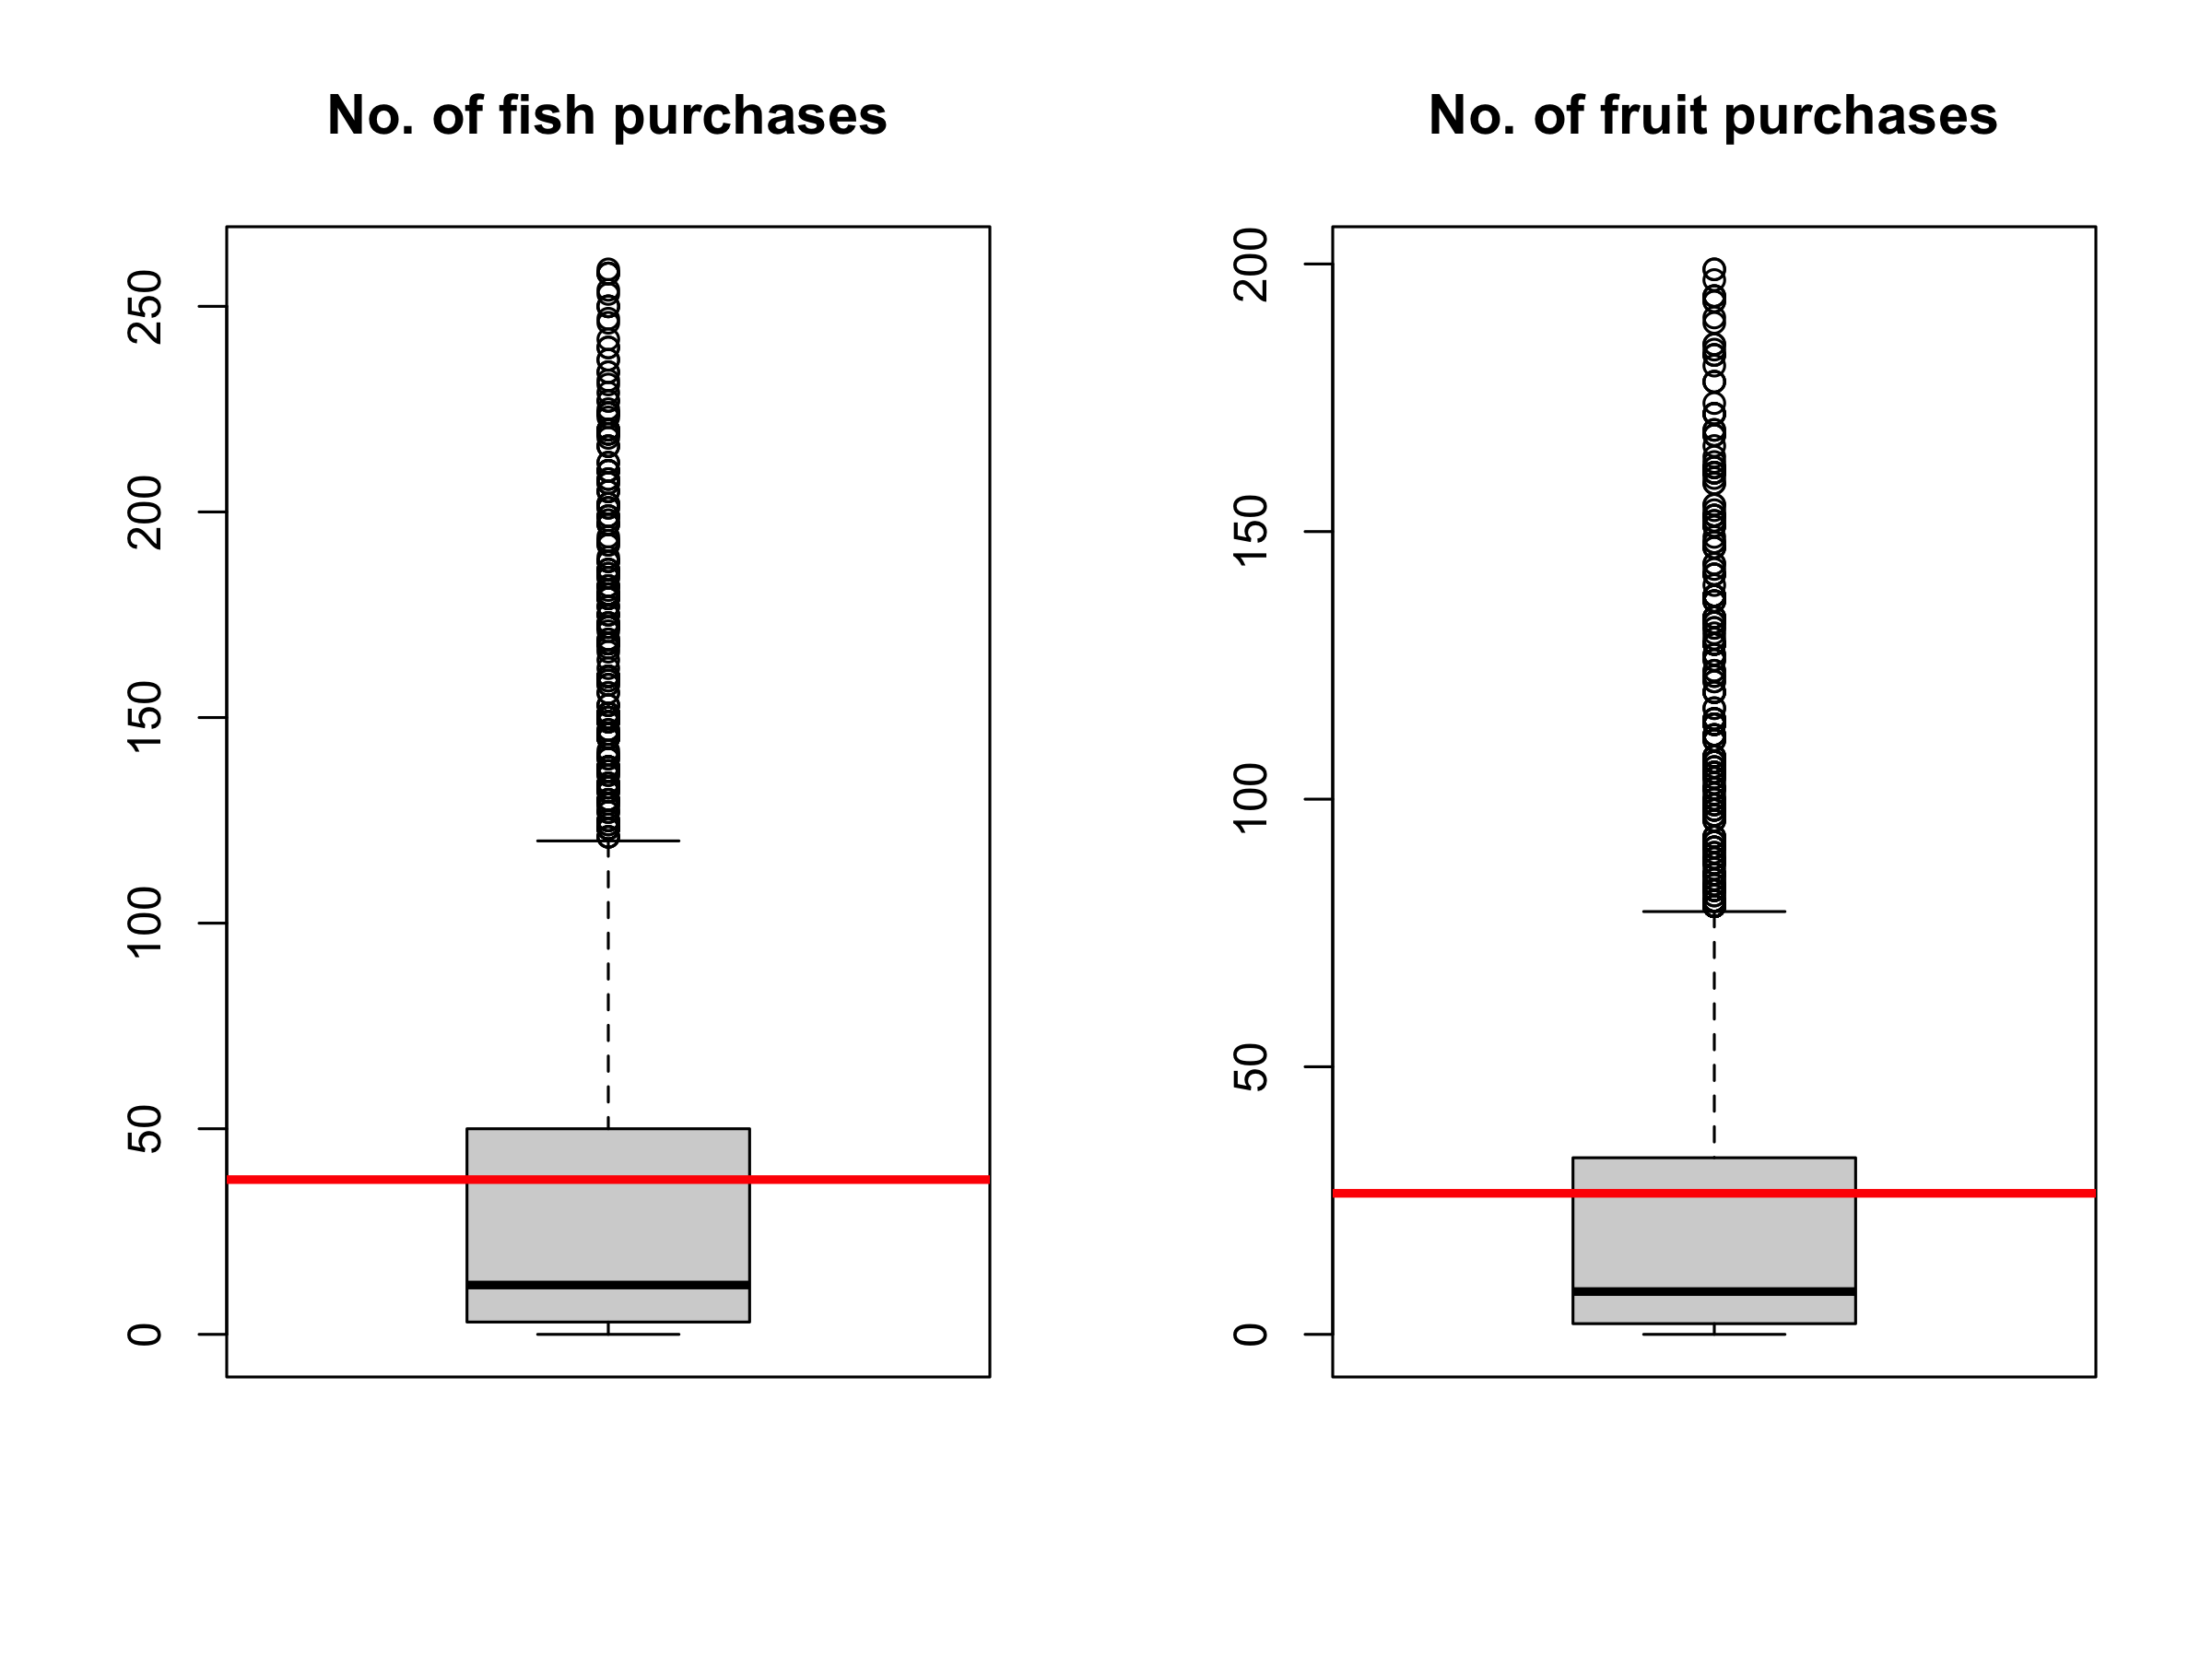
\includegraphics{Report_files/figure-pdf/unnamed-chunk-3-1.png}

Our analysis revealed a significant presence of outliers in all four
food item categories based on the boxplots. The boxes within the plots
represent the interquartile range (IQR), encompassing the middle 50\% of
the data. Values falling outside the whiskers extending from the boxes
are considered potential outliers. \textbf{We have made a horizontal red
line along mean and which clearly shows that our mean and median differ
from each other quite a bit in each food items.}

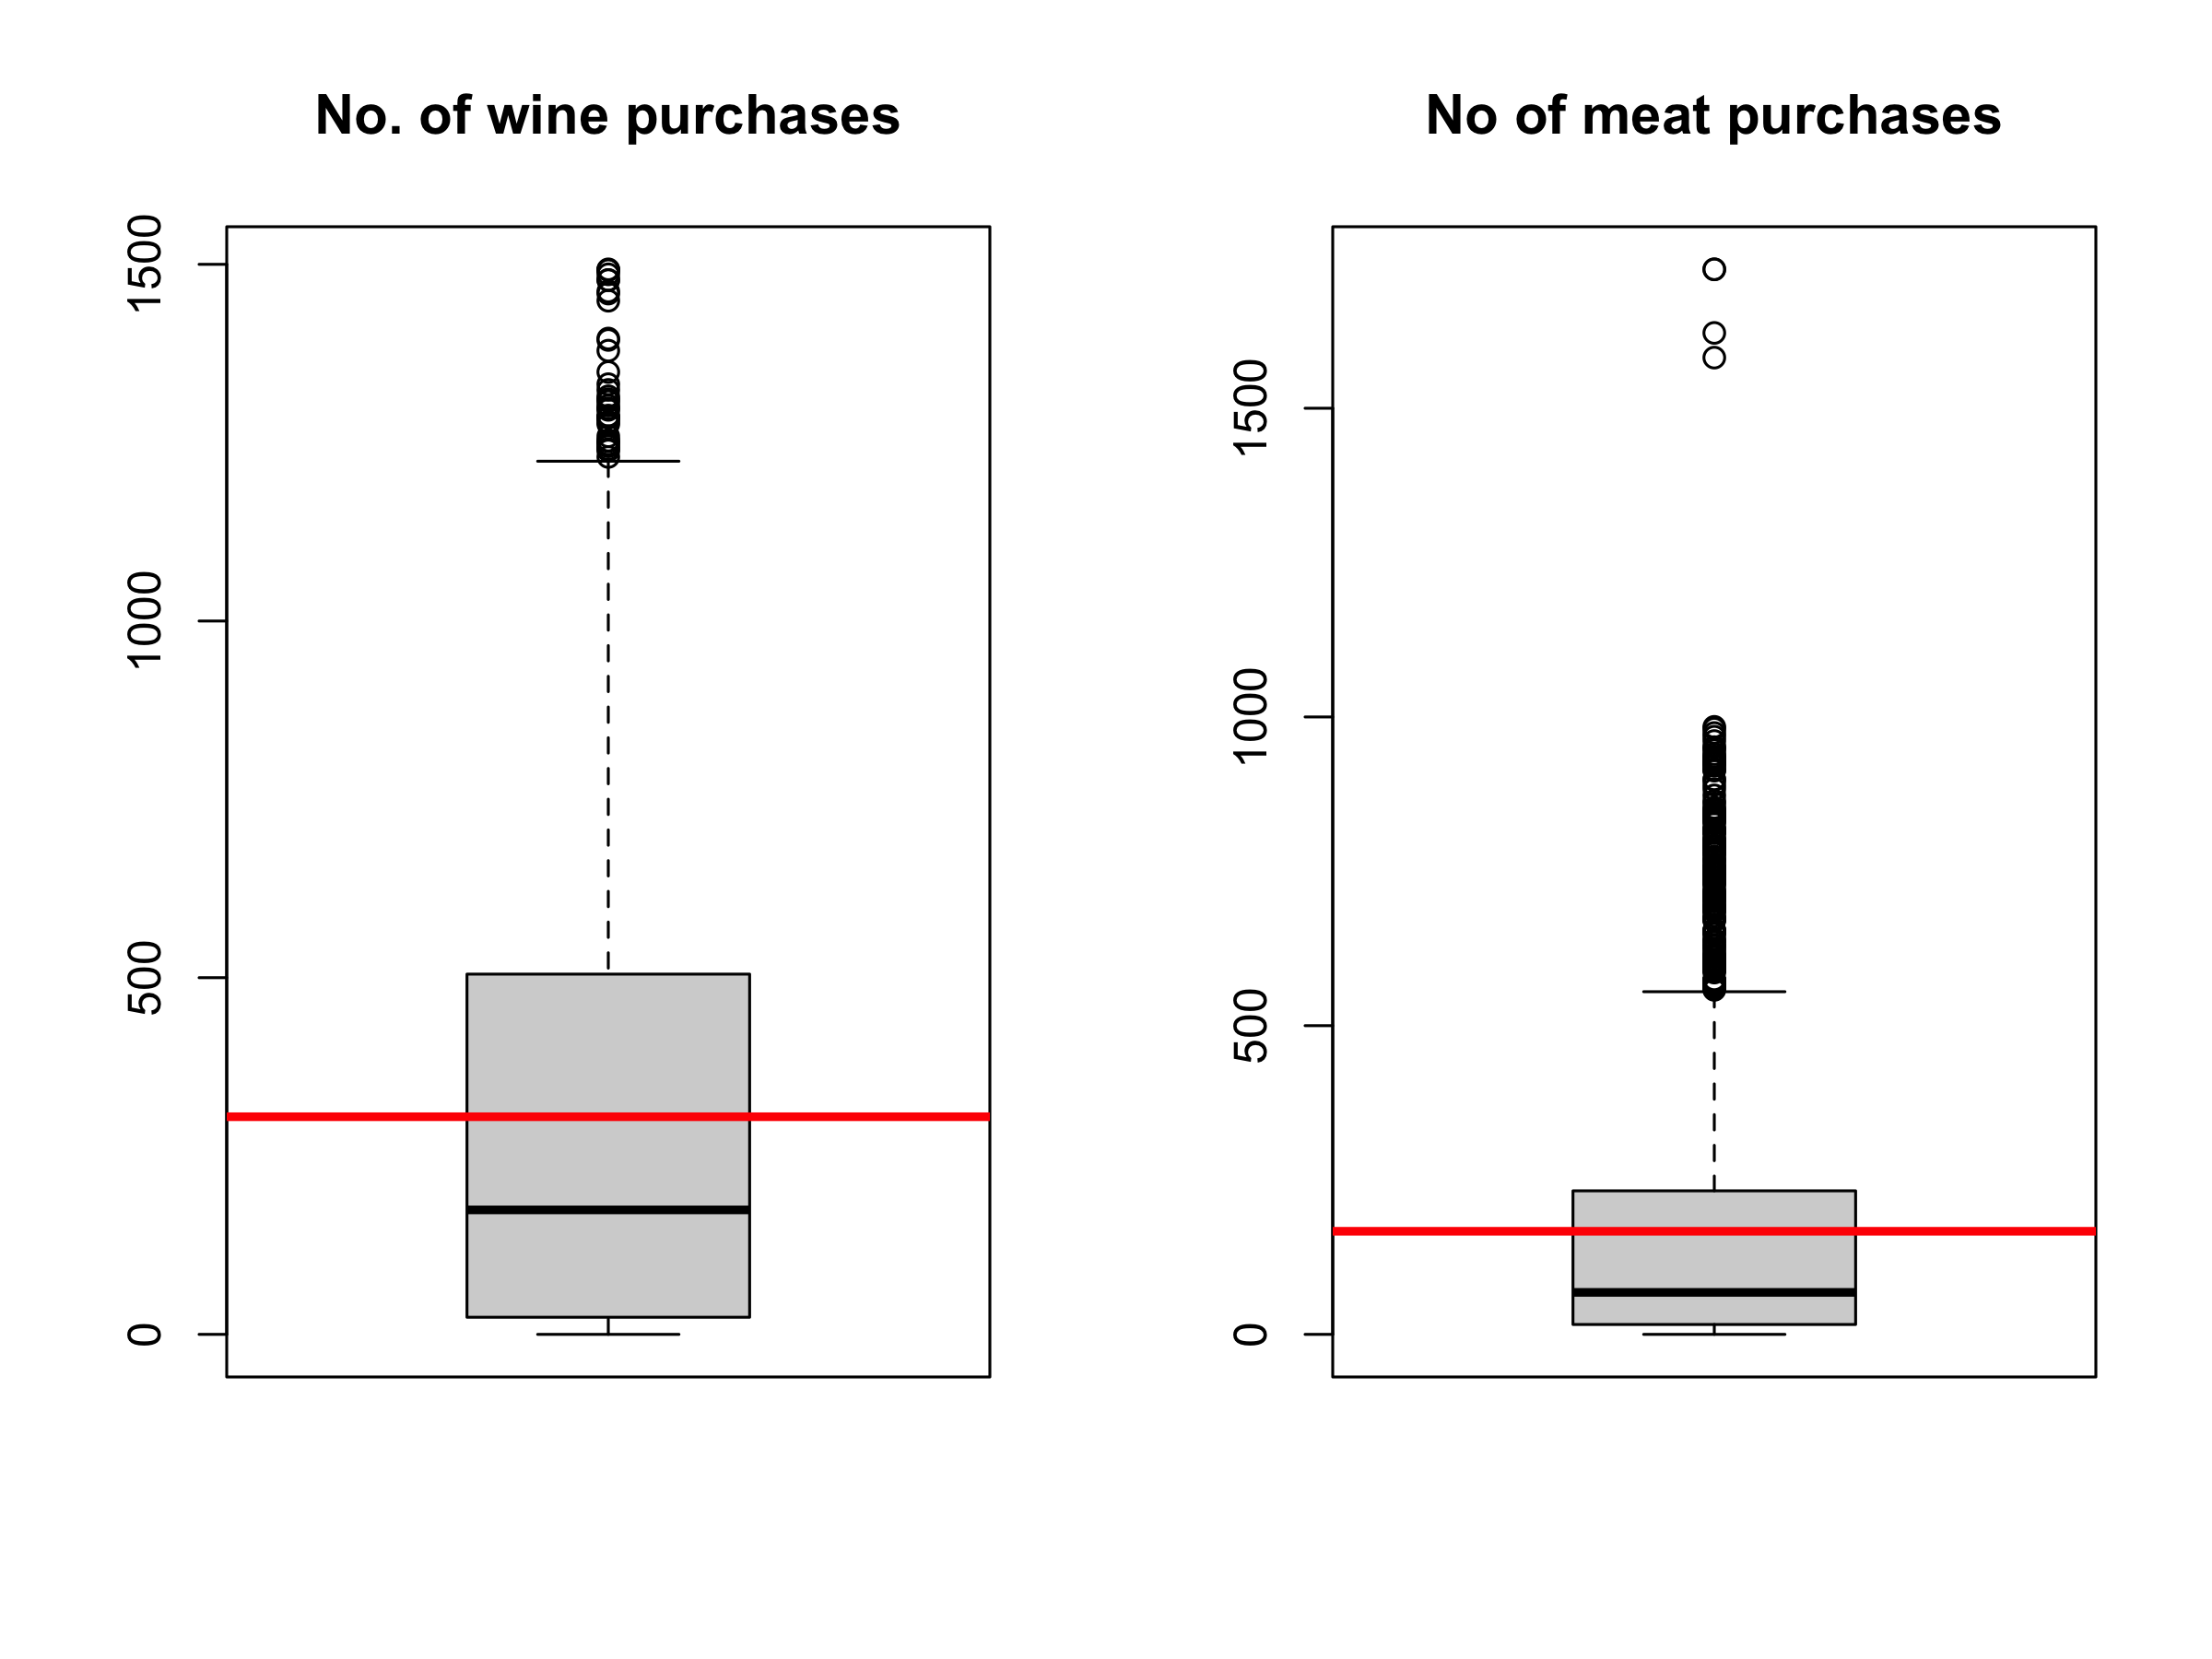
\includegraphics{Report_files/figure-pdf/unnamed-chunk-4-1.png}

\hypertarget{mosaic-plots-and-our-data}{%
\section{1.2 Mosaic Plots and Our
Data}\label{mosaic-plots-and-our-data}}

In this case, the mosaic plot will depict the proportion of individuals
within each education level category (e.g.~2nd cycle, basic, graduation,
masters, PhD) segmented by their marital status (e.g., married, single,
together, divorced). The size of each rectangle will visually represent
the percentage of people in that specific education level and marital
status combination.

\begin{verbatim}
            
             Absurd Alone Divorced Married Single Together Widow YOLO
  2n Cycle        0     0       23      80     36       56     5    0
  Basic           0     0        1      20     18       14     1    0
  Graduation      1     1      119     429    246      285    35    0
  Master          1     1       37     138     75      102    11    0
  PhD             0     1       52     190     96      116    24    2
\end{verbatim}

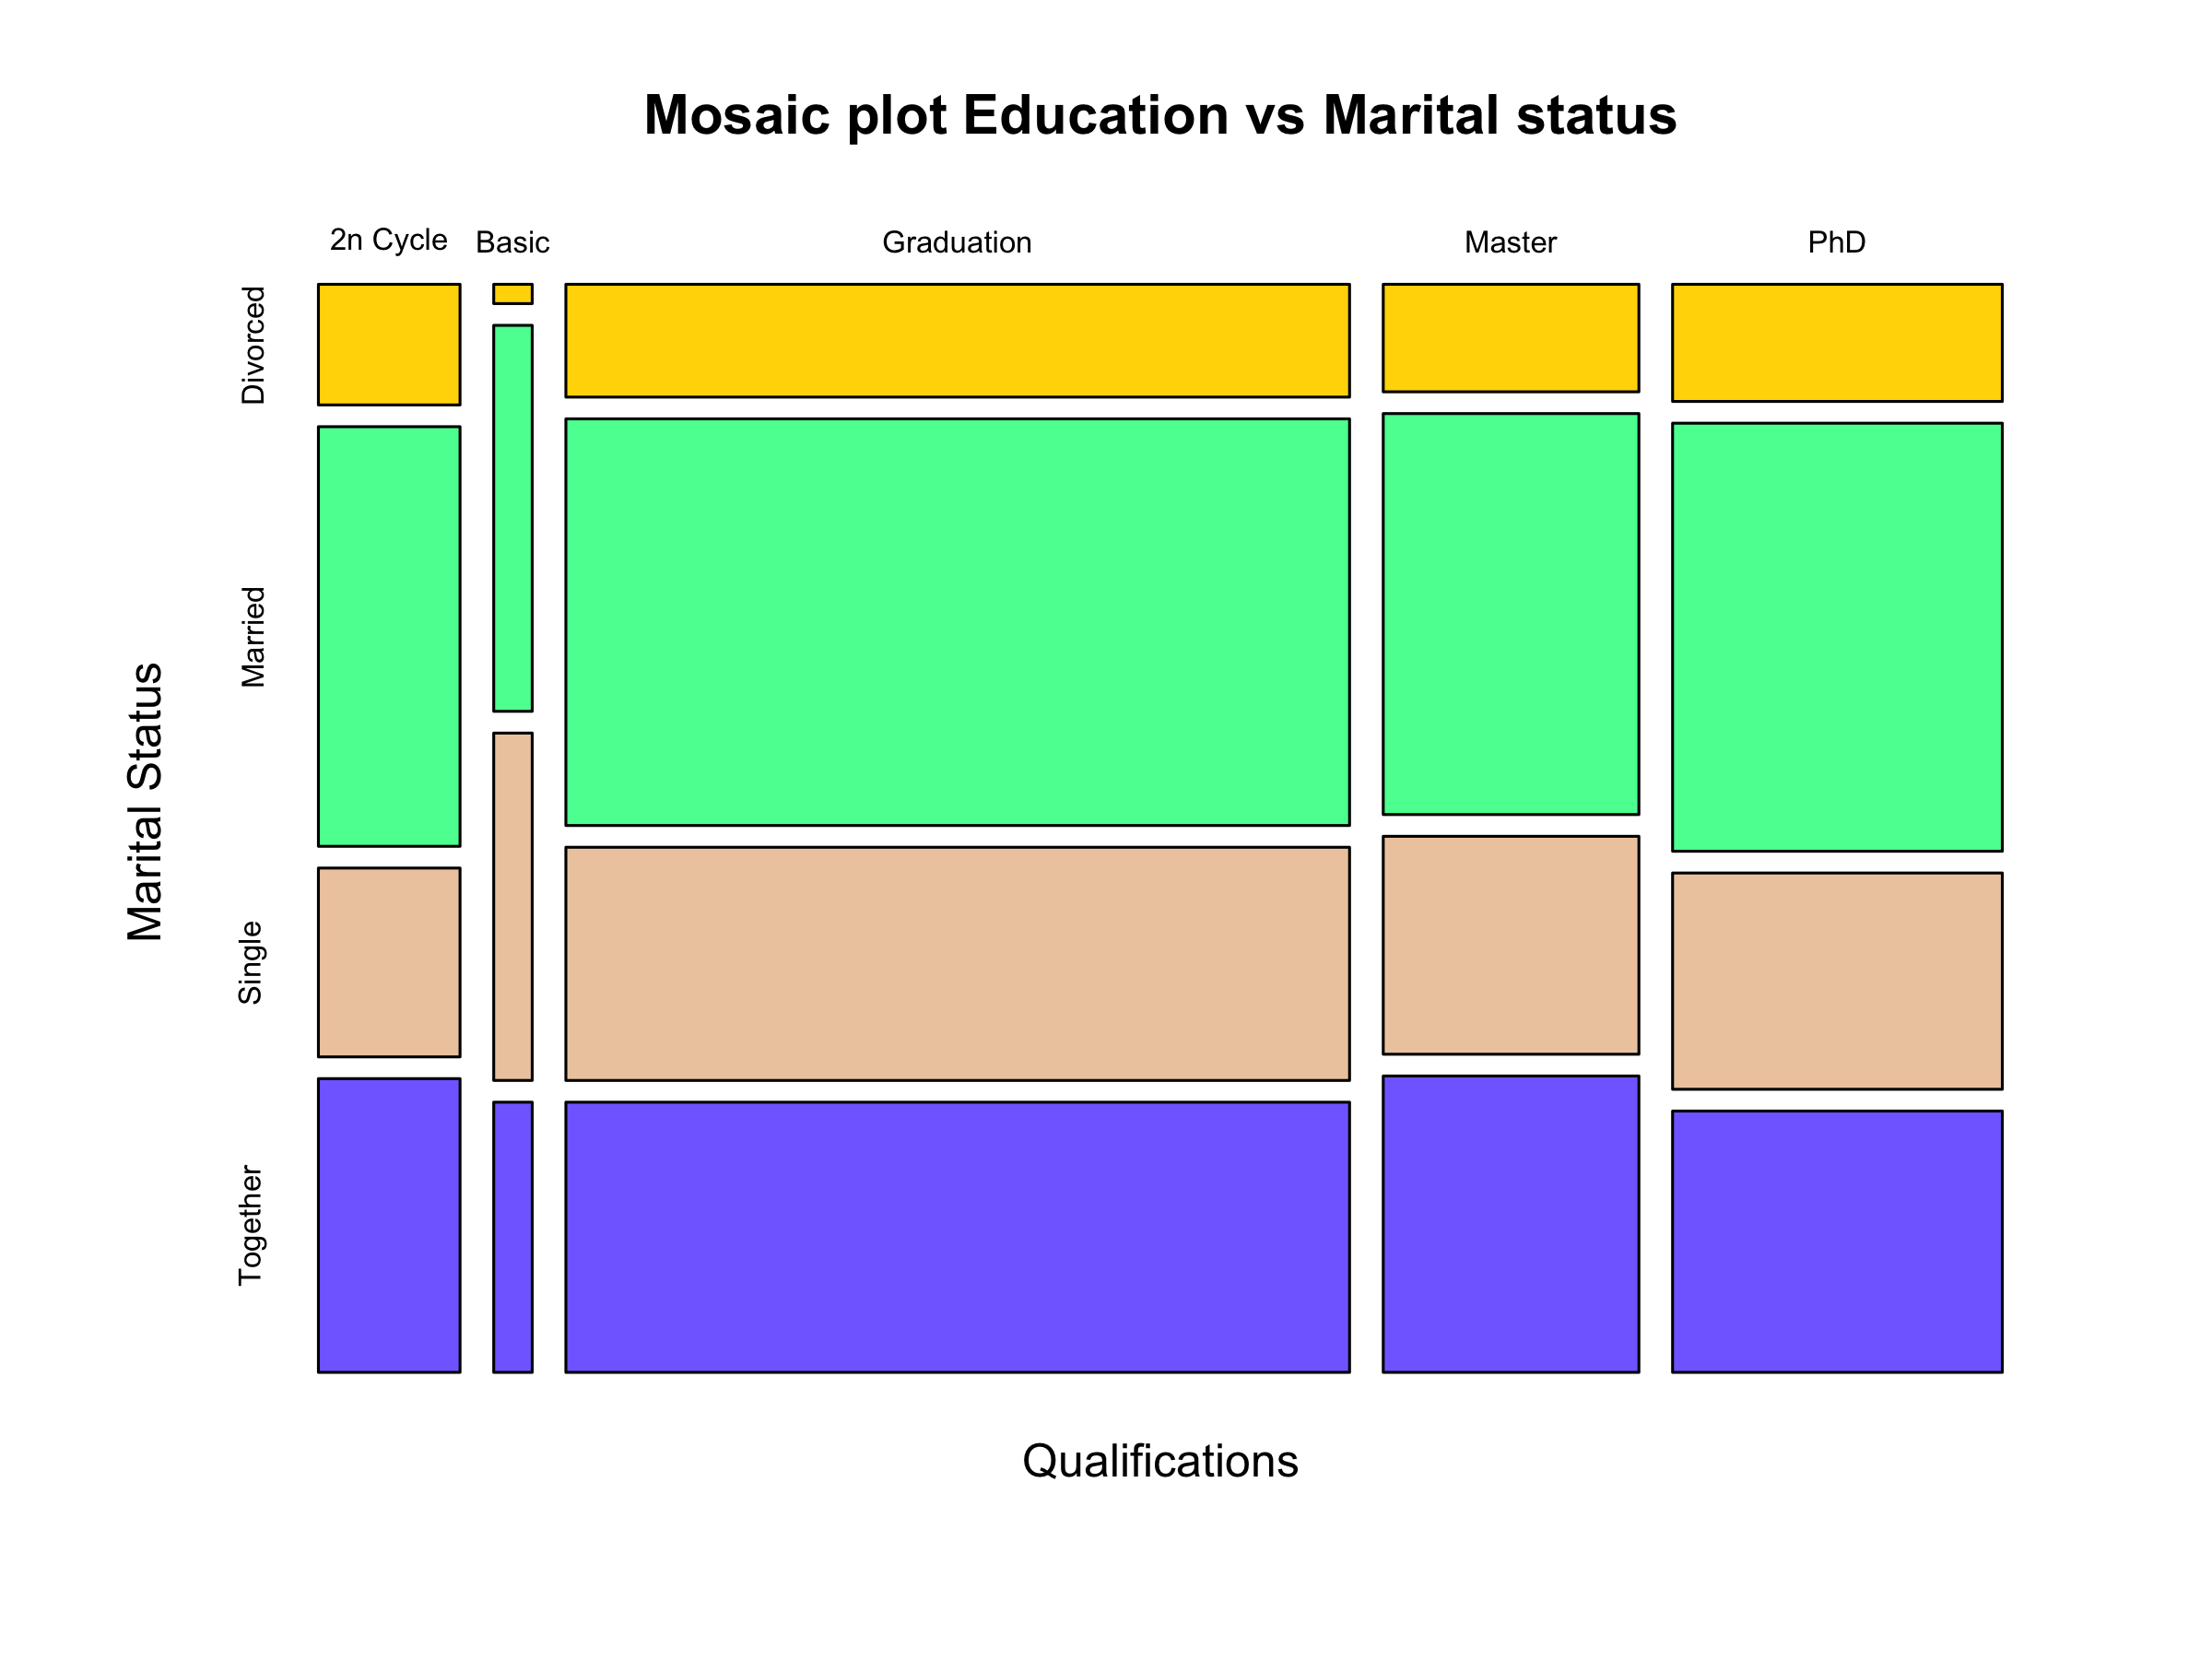
\includegraphics{Report_files/figure-pdf/unnamed-chunk-5-1.png}

\newpage

\hypertarget{correlation-plot}{%
\section{1.3 Correlation Plot}\label{correlation-plot}}

\hypertarget{plot-1-correlations-between-all-products}{%
\subsection{1.3.1 Plot 1: Correlations Between All
Products}\label{plot-1-correlations-between-all-products}}

This correlation plot reveals a positive correlation (likely depicted by
blue color) between all the products, including seats, fruits, wine,
meat, fish, and gold. Positive correlation signifies that when the value
of one product increases, the values of other products tend to increase
as well, and vice versa.

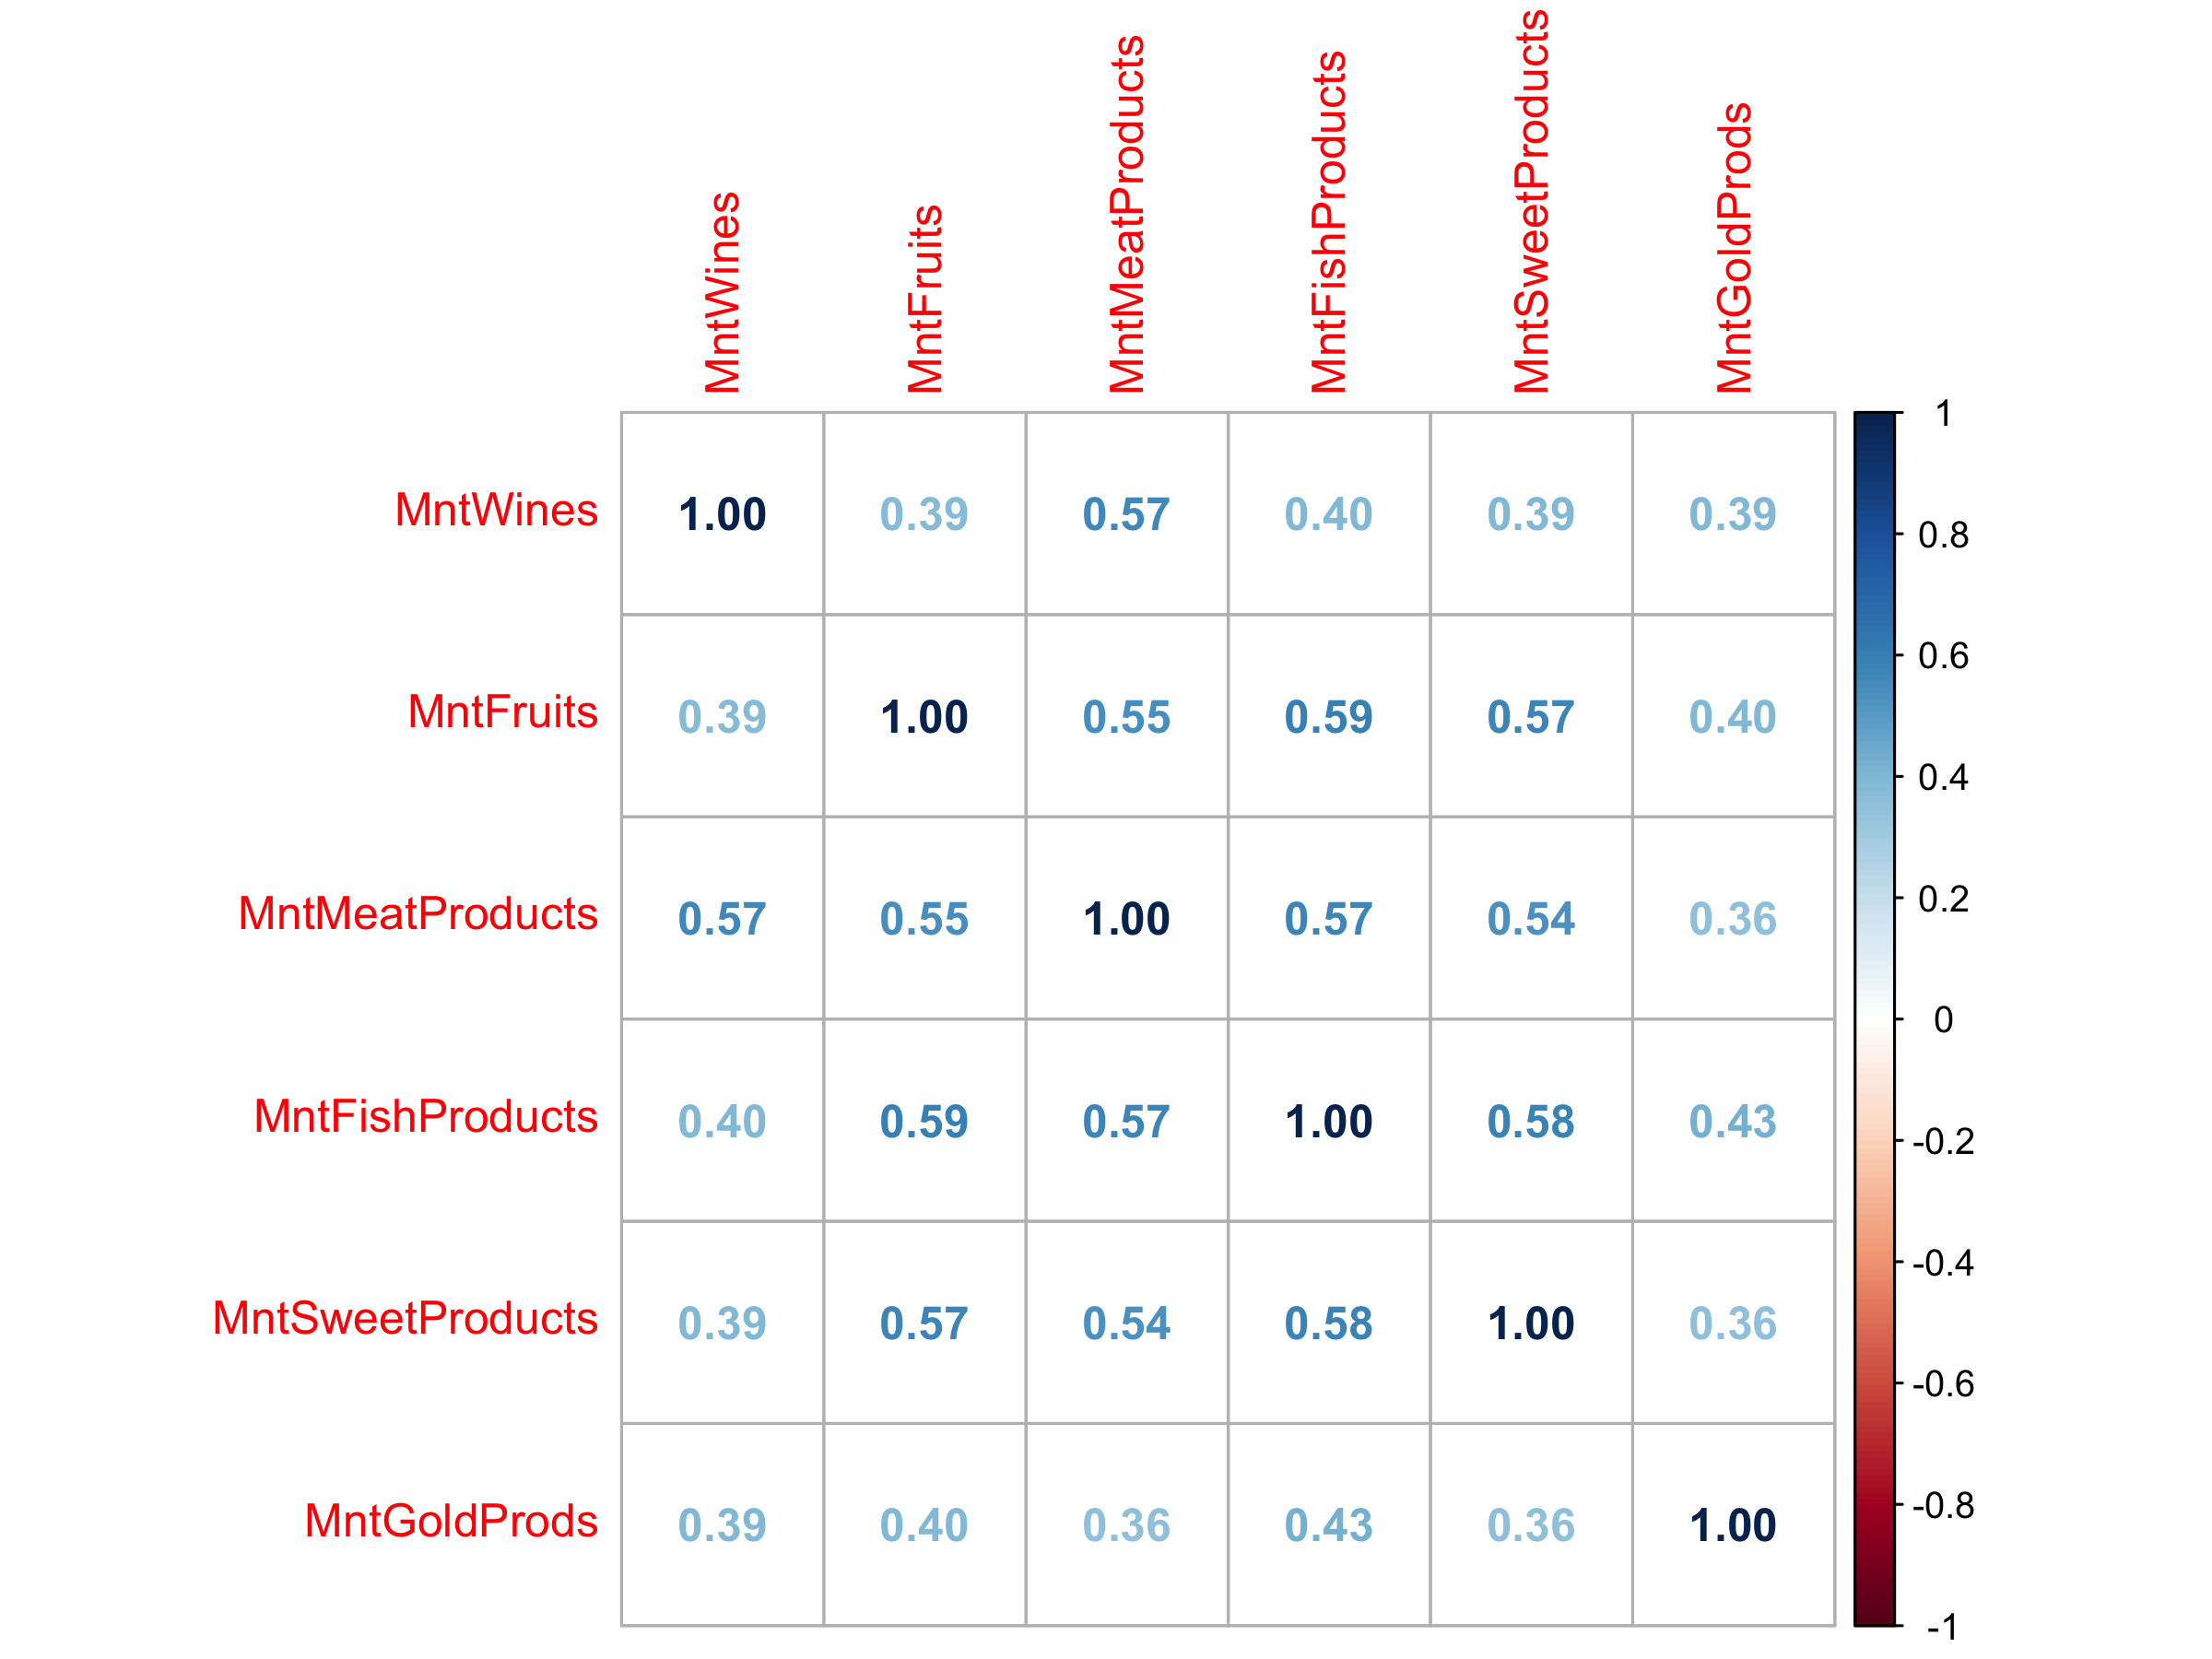
\includegraphics{Report_files/figure-pdf/unnamed-chunk-6-1.png}

\hypertarget{plot-2-correlations-between-purchase-sources}{%
\subsection{1.3.2 Plot 2: Correlations Between Purchase
Sources}\label{plot-2-correlations-between-purchase-sources}}

This correlation plot examines the relationship between purchase
sources, such as web, catalog, store, and potentially others. \textbf{We
can see a negative correlation between the Number of web visits and
(Number of store and catalog purchases) and we can infer from it that
tech savvy people prefer less to go physically to stores }

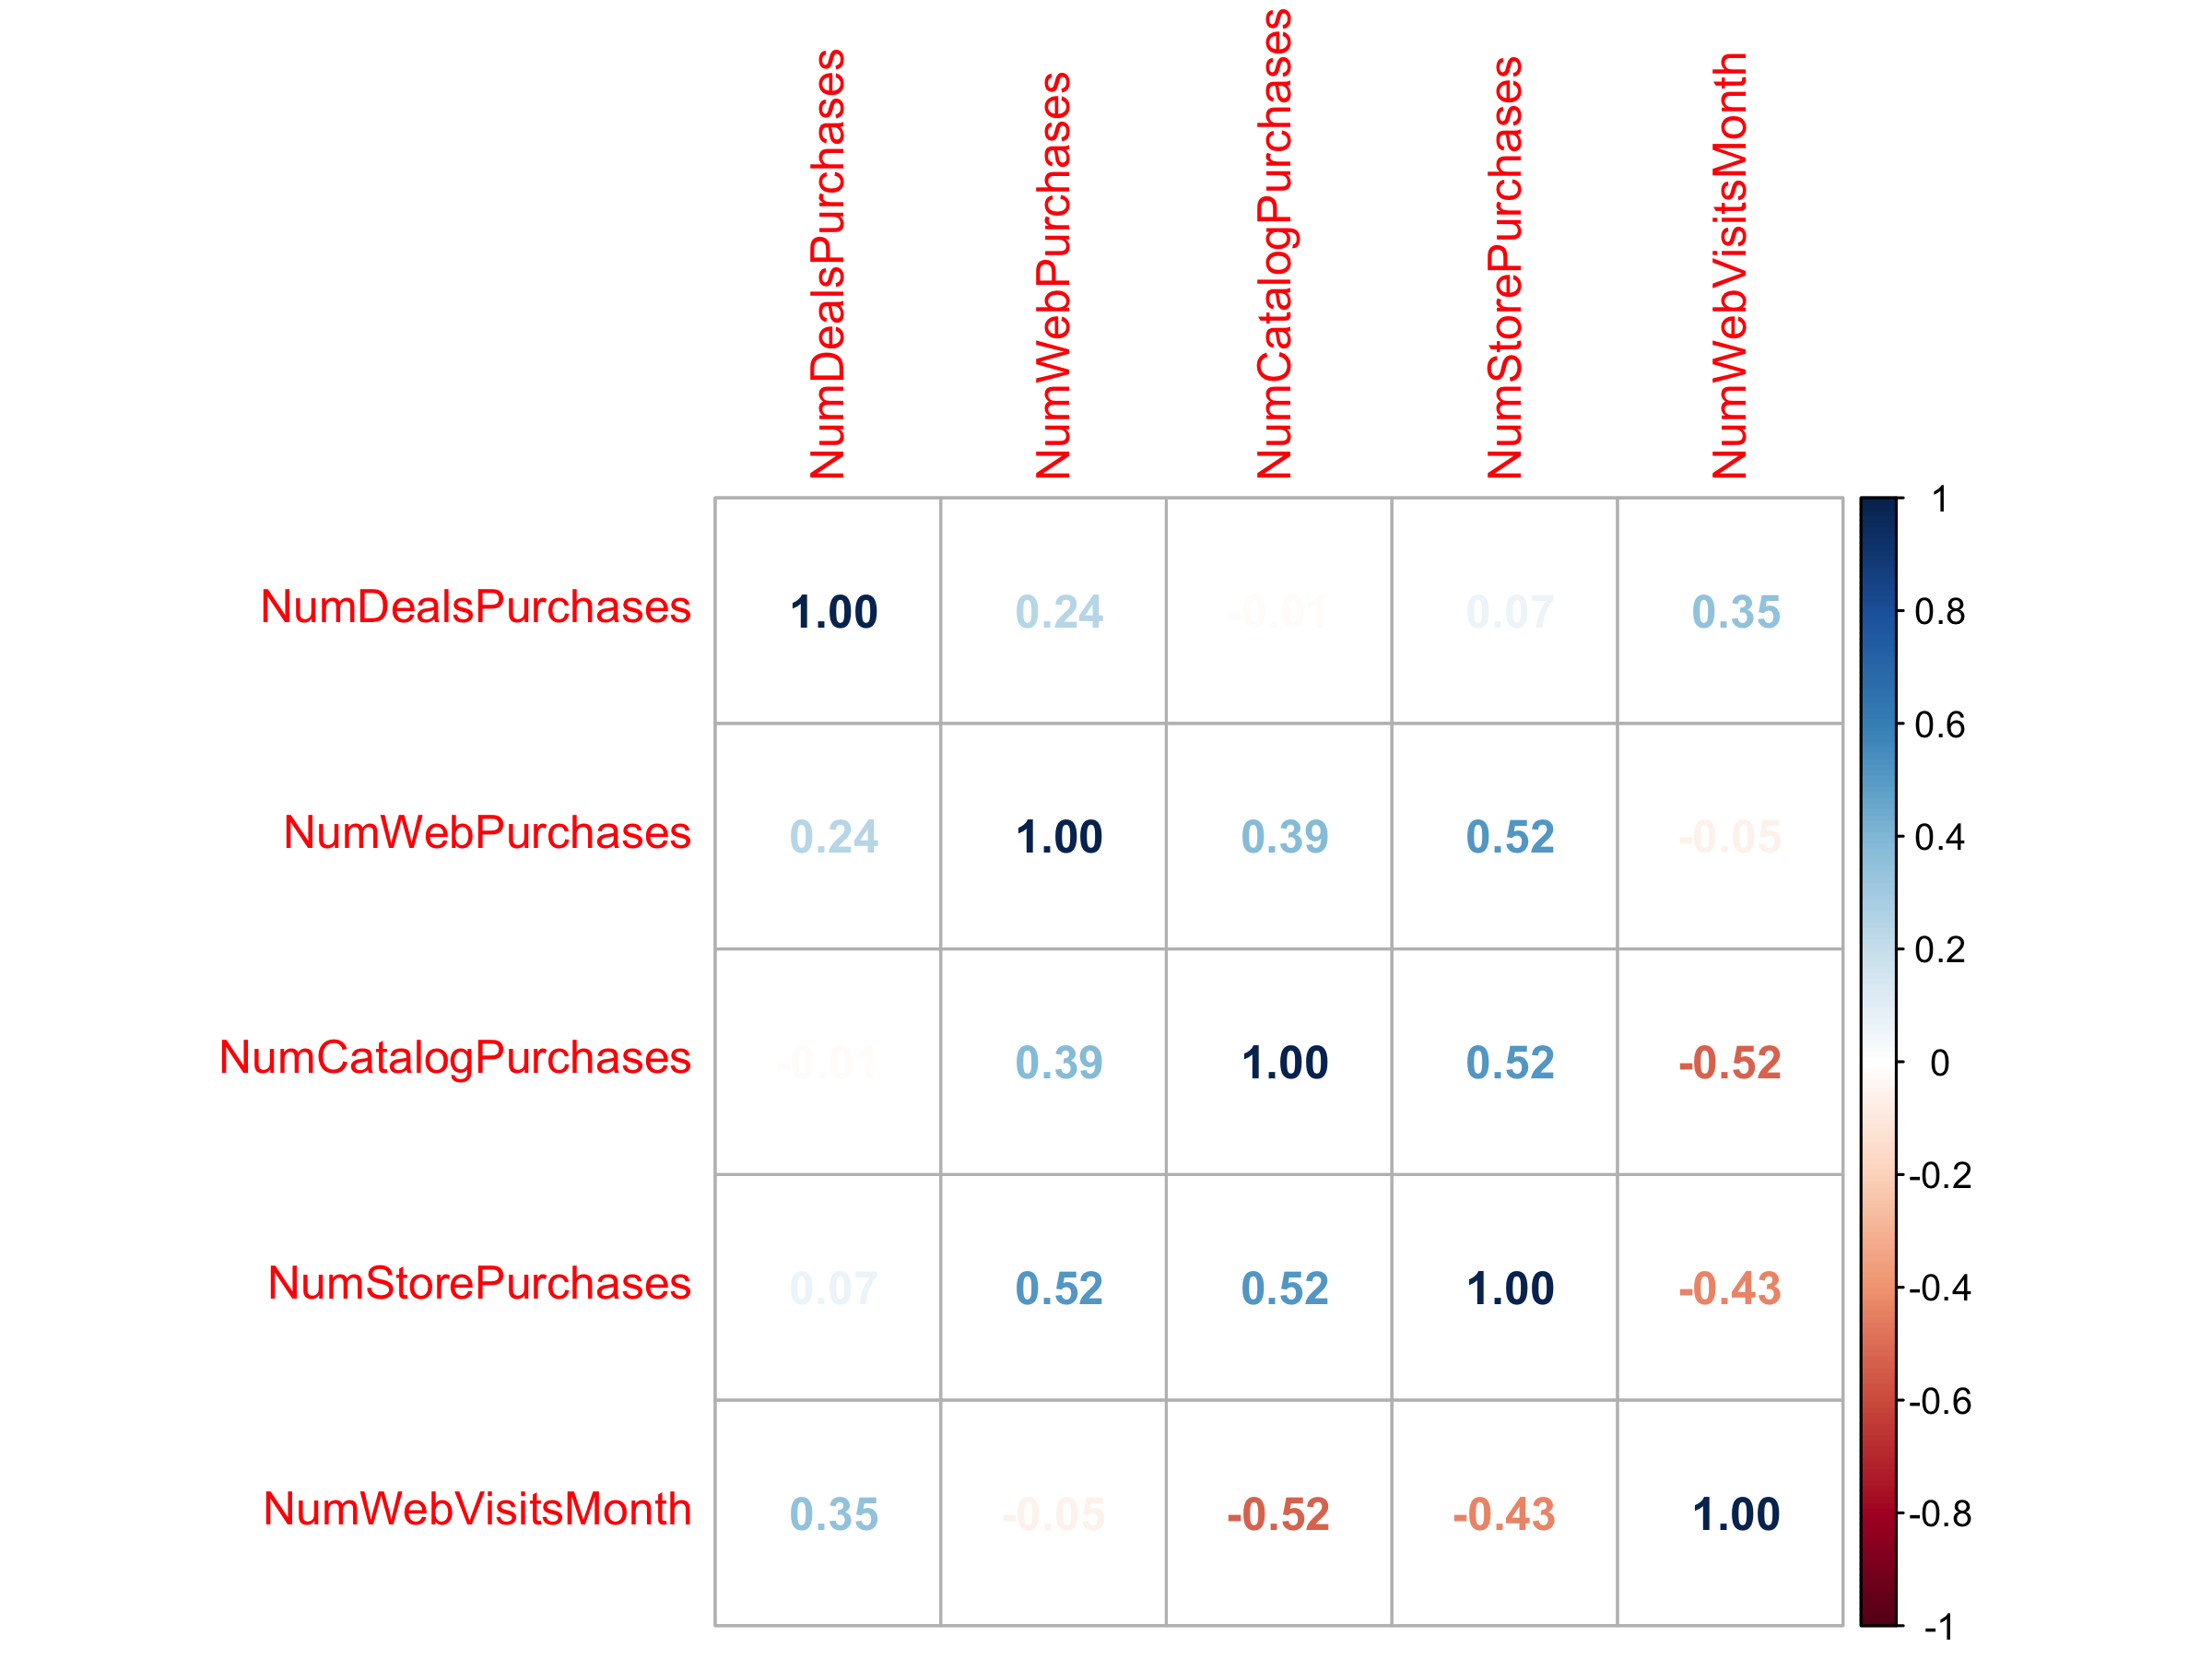
\includegraphics{Report_files/figure-pdf/unnamed-chunk-7-1.png}

\hypertarget{scatter-plot-between-premium-products}{%
\subsection{1.4 Scatter plot between premium
products}\label{scatter-plot-between-premium-products}}

\hypertarget{principal-component-analysis}{%
\section{2. Principal Component
Analysis}\label{principal-component-analysis}}

The data we have was high dimensional data with multiple columns which
led to difficulty in organizing and analyzing the various components. We
thus used PCA to reduce the dimensionalty of our data.

First step was to clean and filter out the data which was not required.
We removed the categorical variables as they were increasing the
complexity of the data. Further, we removed the columns with zero
variance and the rows with missing values. Following is the head of the
cleaned data:

\begin{verbatim}
  X   ID Year_Birth Income Kidhome Teenhome Recency MntWines MntFruits
1 1 5524       1957  58138       0        0      58      635        88
2 2 2174       1954  46344       1        1      38       11         1
3 3 4141       1965  71613       0        0      26      426        49
4 4 6182       1984  26646       1        0      26       11         4
5 5 5324       1981  58293       1        0      94      173        43
  MntMeatProducts MntFishProducts MntSweetProducts MntGoldProds
1             546             172               88           88
2               6               2                1            6
3             127             111               21           42
4              20              10                3            5
5             118              46               27           15
  NumDealsPurchases NumWebPurchases NumCatalogPurchases NumStorePurchases
1                 3               8                  10                 4
2                 2               1                   1                 2
3                 1               8                   2                10
4                 2               2                   0                 4
5                 5               5                   3                 6
  NumWebVisitsMonth AcceptedCmp3 AcceptedCmp4 AcceptedCmp5 AcceptedCmp1
1                 7            0            0            0            0
2                 5            0            0            0            0
3                 4            0            0            0            0
4                 6            0            0            0            0
5                 5            0            0            0            0
  AcceptedCmp2 Complain Response
1            0        0        1
2            0        0        0
3            0        0        0
4            0        0        0
5            0        0        0
\end{verbatim}

As we can see, there are 24 columns even after cleaning the data, which
shows the high dimensionalty.

Then, we performed PCA which gave the following result:

\begin{verbatim}
Importance of components:
                          PC1     PC2     PC3     PC4     PC5    PC6     PC7
Standard deviation     2.5578 1.42646 1.38040 1.18565 1.05513 1.0198 1.01137
Proportion of Variance 0.2617 0.08139 0.07622 0.05623 0.04453 0.0416 0.04091
Cumulative Proportion  0.2617 0.34308 0.41930 0.47553 0.52007 0.5617 0.60258
                           PC8     PC9    PC10    PC11    PC12    PC13    PC14
Standard deviation     0.99824 0.96839 0.92441 0.86997 0.86138 0.81100 0.78243
Proportion of Variance 0.03986 0.03751 0.03418 0.03027 0.02968 0.02631 0.02449
Cumulative Proportion  0.64244 0.67995 0.71413 0.74441 0.77409 0.80039 0.82488
                          PC15    PC16    PC17    PC18    PC19   PC20    PC21
Standard deviation     0.76266 0.74942 0.71948 0.68018 0.65337 0.6384 0.61253
Proportion of Variance 0.02327 0.02247 0.02071 0.01851 0.01708 0.0163 0.01501
Cumulative Proportion  0.84815 0.87061 0.89132 0.90983 0.92690 0.9432 0.95821
                          PC22    PC23    PC24    PC25
Standard deviation     0.56232 0.54660 0.48409 0.44204
Proportion of Variance 0.01265 0.01195 0.00937 0.00782
Cumulative Proportion  0.97086 0.98281 0.99218 1.00000
\end{verbatim}

Below is the plot of the PCA analysis and the cumulative variance of the
components:

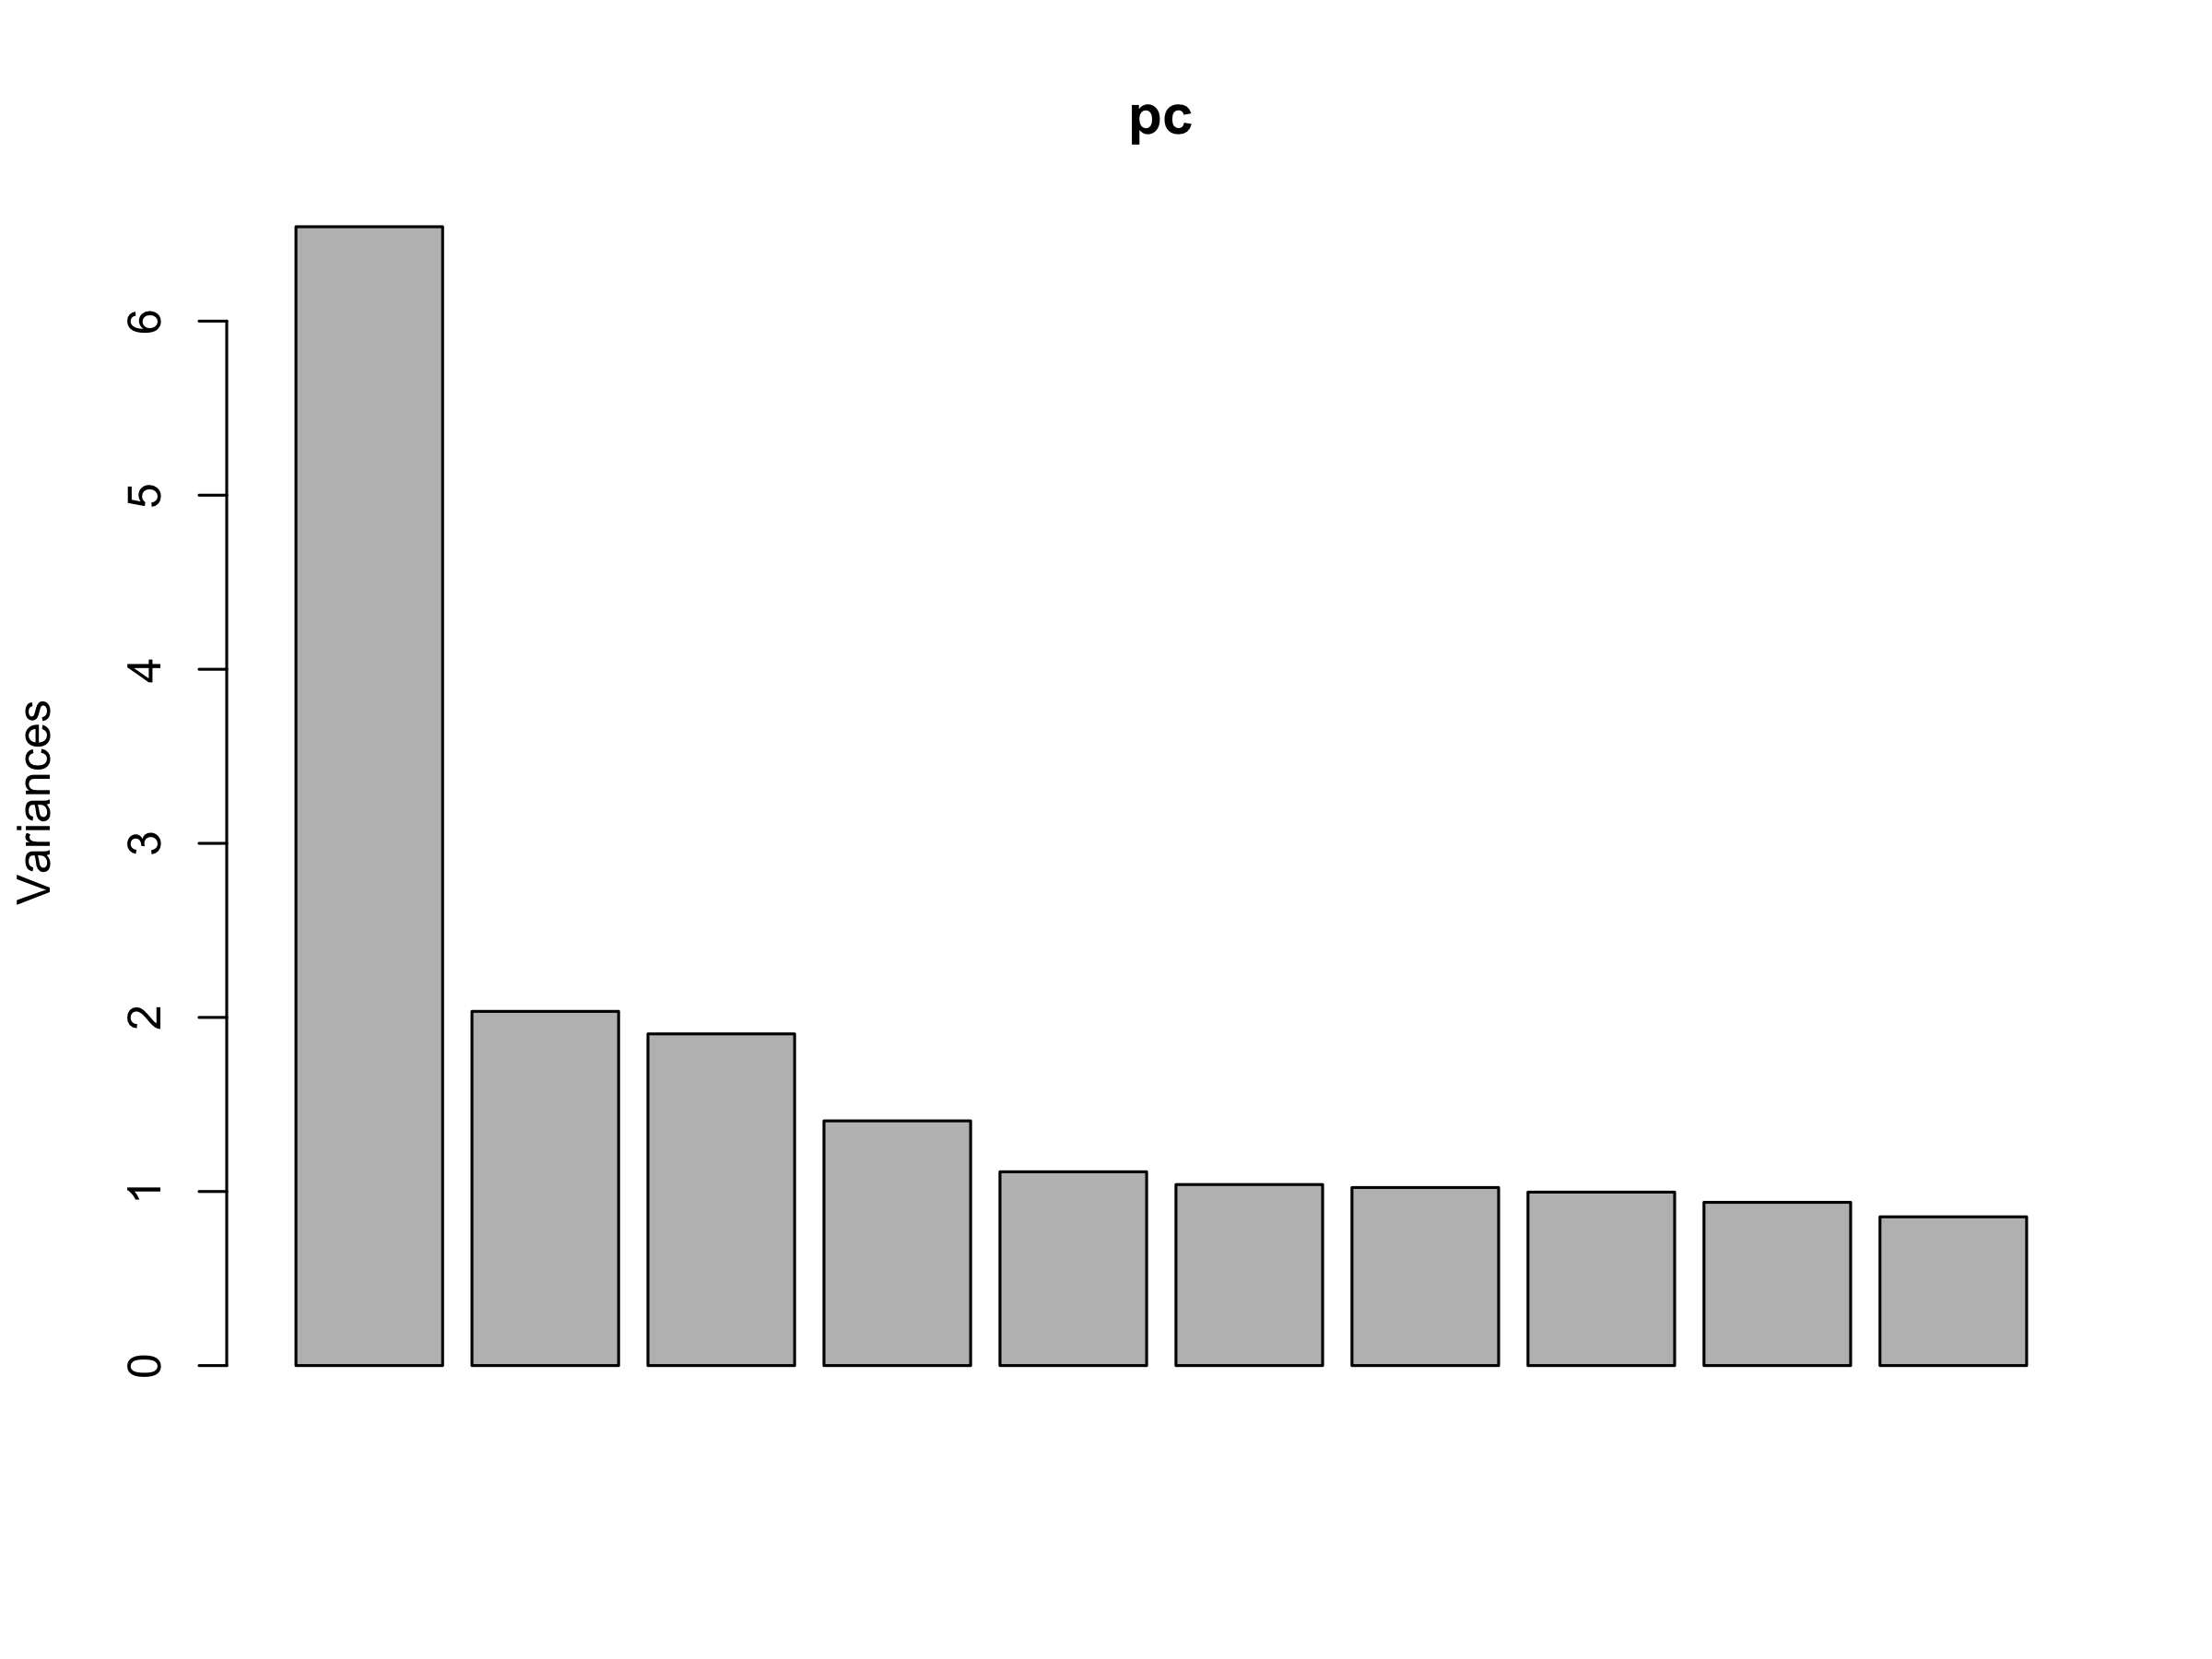
\includegraphics{Report_files/figure-pdf/unnamed-chunk-10-1.png}

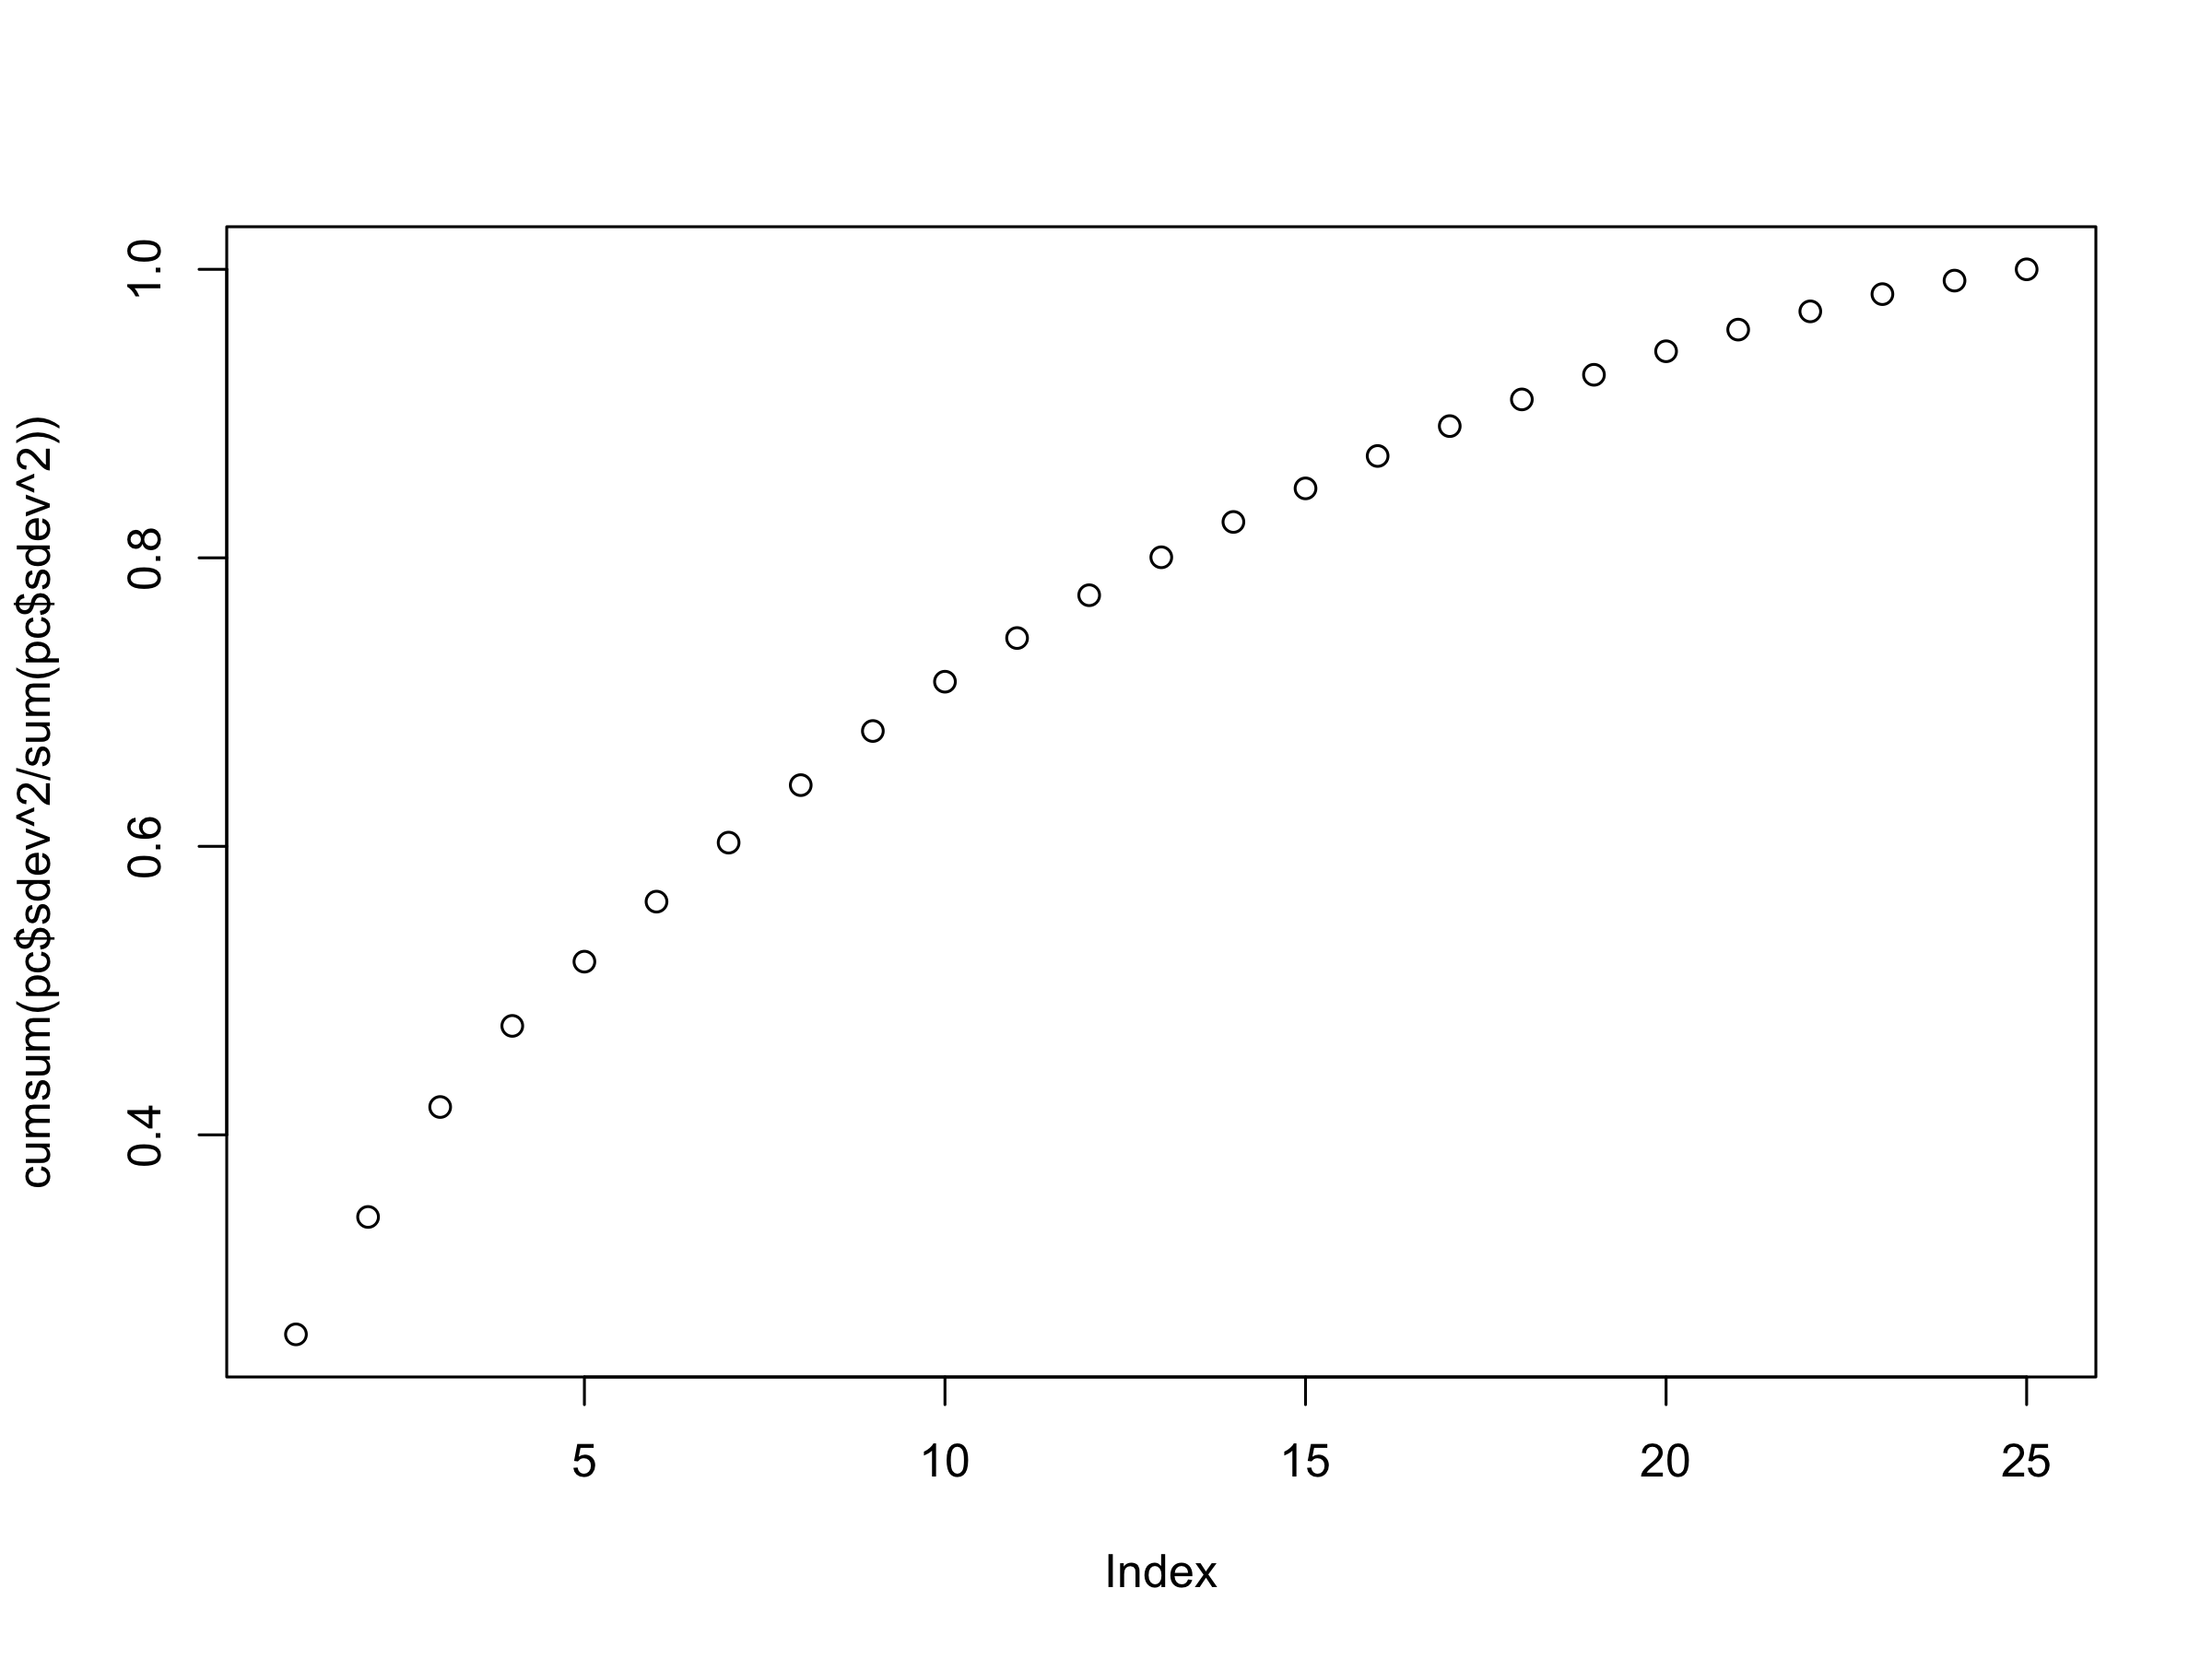
\includegraphics{Report_files/figure-pdf/unnamed-chunk-11-1.png}

Thus, around 13 components are able to explain 80\% variability in the
data.

Below is a plot of the relationship between the first two components
after PCA.

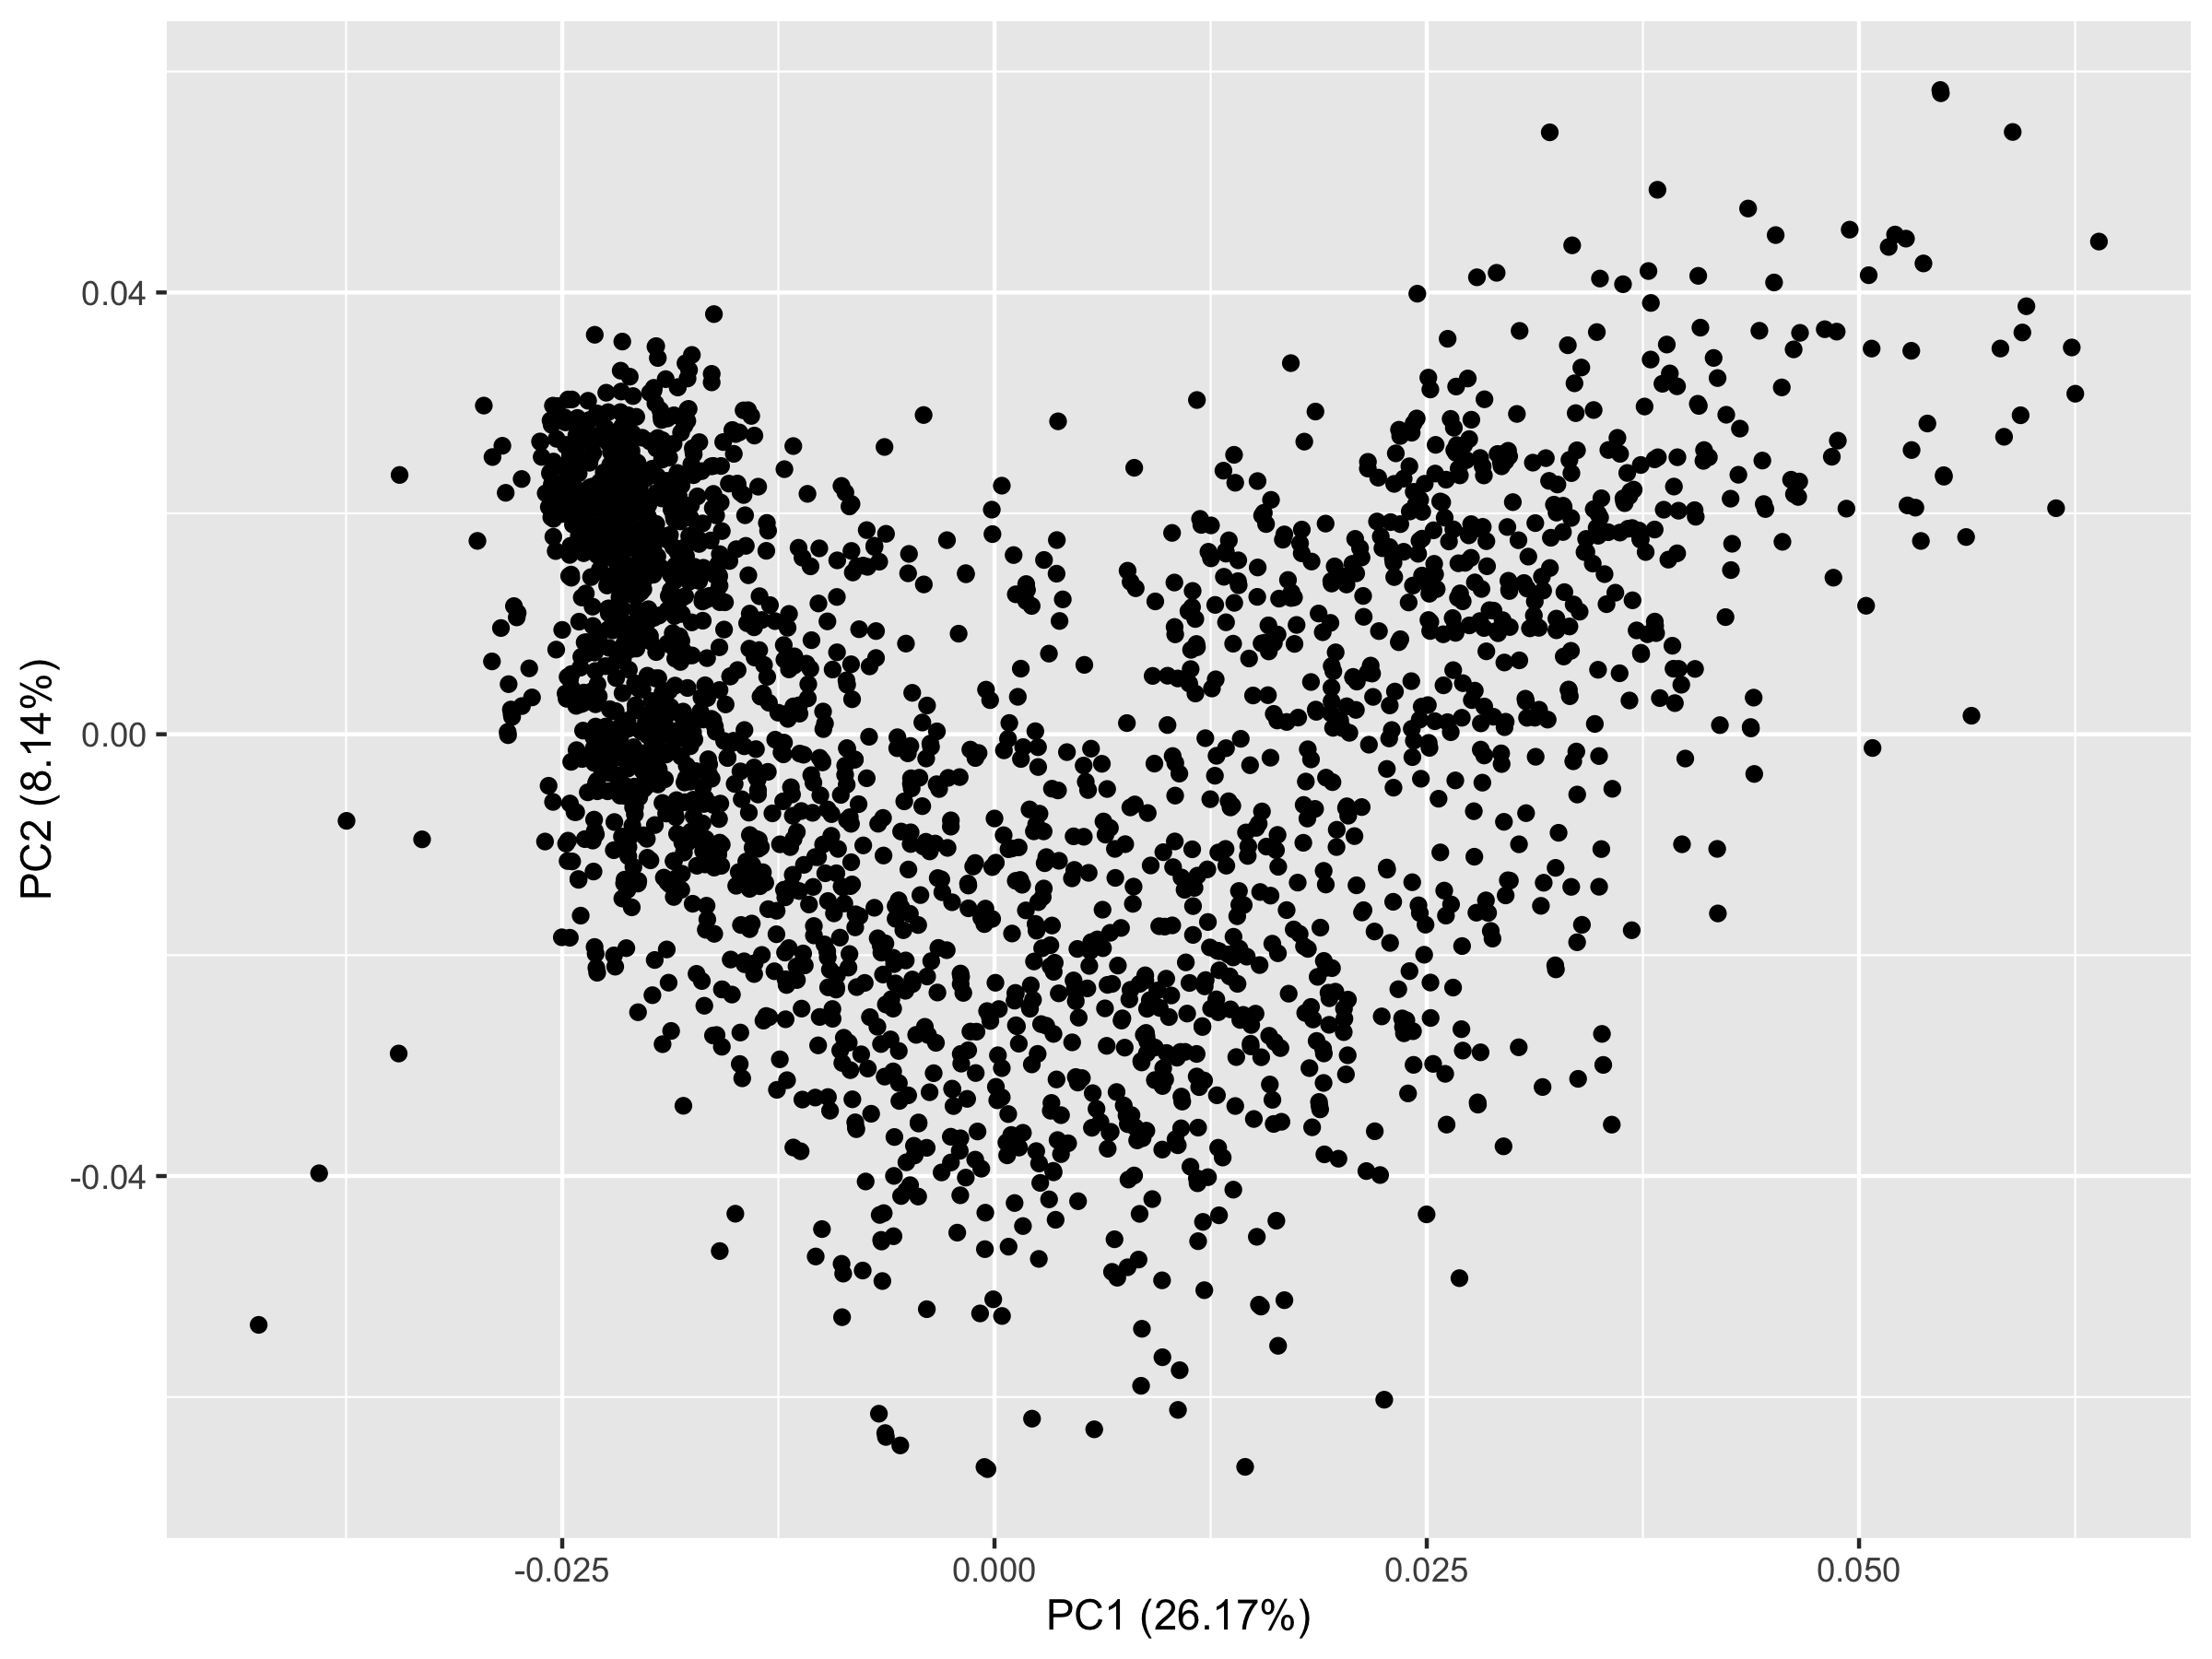
\includegraphics{Report_files/figure-pdf/unnamed-chunk-12-1.png}

Thus, with the help of PCA we can reduce the data with 24 columns to
upto 13 columns and still explain 80\% variability in the data.

=======

\begin{quote}
\begin{quote}
\begin{quote}
\begin{quote}
\begin{quote}
\begin{quote}
\begin{quote}
538b818351843ff58216a43c10b7beb63ea3990e
\end{quote}
\end{quote}
\end{quote}
\end{quote}
\end{quote}
\end{quote}
\end{quote}

\hypertarget{principal-component-analysis-1}{%
\subsection{Principal Component
Analysis}\label{principal-component-analysis-1}}

The data we have was high dimensional data with multiple columns which
led to difficulty in organizing and analyzing the various components. We
thus used PCA to reduce the dimensionalty of our data.

First step was to clean and filter out the data which was not required.
We removed the categorical variables as they were increasing the
complexity of the data. Further, we removed the columns with zero
variance and the rows with missing values. Following is the head of the
cleaned data:

\begin{verbatim}
# A tibble: 5 x 24
     ID Year_Birth Income Kidhome Teenhome Recency MntWines MntFruits
  <dbl>      <dbl>  <dbl>   <dbl>    <dbl>   <dbl>    <dbl>     <dbl>
1  5524       1957  58138       0        0      58      635        88
2  2174       1954  46344       1        1      38       11         1
3  4141       1965  71613       0        0      26      426        49
4  6182       1984  26646       1        0      26       11         4
5  5324       1981  58293       1        0      94      173        43
# i 16 more variables: MntMeatProducts <dbl>, MntFishProducts <dbl>,
#   MntSweetProducts <dbl>, MntGoldProds <dbl>, NumDealsPurchases <dbl>,
#   NumWebPurchases <dbl>, NumCatalogPurchases <dbl>, NumStorePurchases <dbl>,
#   NumWebVisitsMonth <dbl>, AcceptedCmp3 <dbl>, AcceptedCmp4 <dbl>,
#   AcceptedCmp5 <dbl>, AcceptedCmp1 <dbl>, AcceptedCmp2 <dbl>, Complain <dbl>,
#   Response <dbl>
\end{verbatim}

As we can see, there are 24 columns even after cleaning the data, which
shows the high dimensionalty.

Then, we performed PCA which gave the following result:

\begin{verbatim}
Importance of components:
                          PC1     PC2     PC3     PC4     PC5     PC6     PC7
Standard deviation     2.5578 1.42624 1.38007 1.18466 1.05487 1.01737 1.00901
Proportion of Variance 0.2726 0.08476 0.07936 0.05848 0.04636 0.04313 0.04242
Cumulative Proportion  0.2726 0.35735 0.43670 0.49518 0.54154 0.58467 0.62709
                           PC8     PC9    PC10    PC11    PC12    PC13    PC14
Standard deviation     0.96948 0.92476 0.87041 0.86141 0.81159 0.78256 0.76318
Proportion of Variance 0.03916 0.03563 0.03157 0.03092 0.02744 0.02552 0.02427
Cumulative Proportion  0.66625 0.70189 0.73345 0.76437 0.79182 0.81733 0.84160
                          PC15    PC16    PC17   PC18    PC19    PC20   PC21
Standard deviation     0.75005 0.72085 0.68036 0.6537 0.63905 0.61263 0.5629
Proportion of Variance 0.02344 0.02165 0.01929 0.0178 0.01702 0.01564 0.0132
Cumulative Proportion  0.86504 0.88669 0.90598 0.9238 0.94080 0.95644 0.9696
                          PC22    PC23    PC24
Standard deviation     0.54660 0.48427 0.44205
Proportion of Variance 0.01245 0.00977 0.00814
Cumulative Proportion  0.98209 0.99186 1.00000
\end{verbatim}

Below is the plot of the PCA analysis and the cumulative variance of the
components:

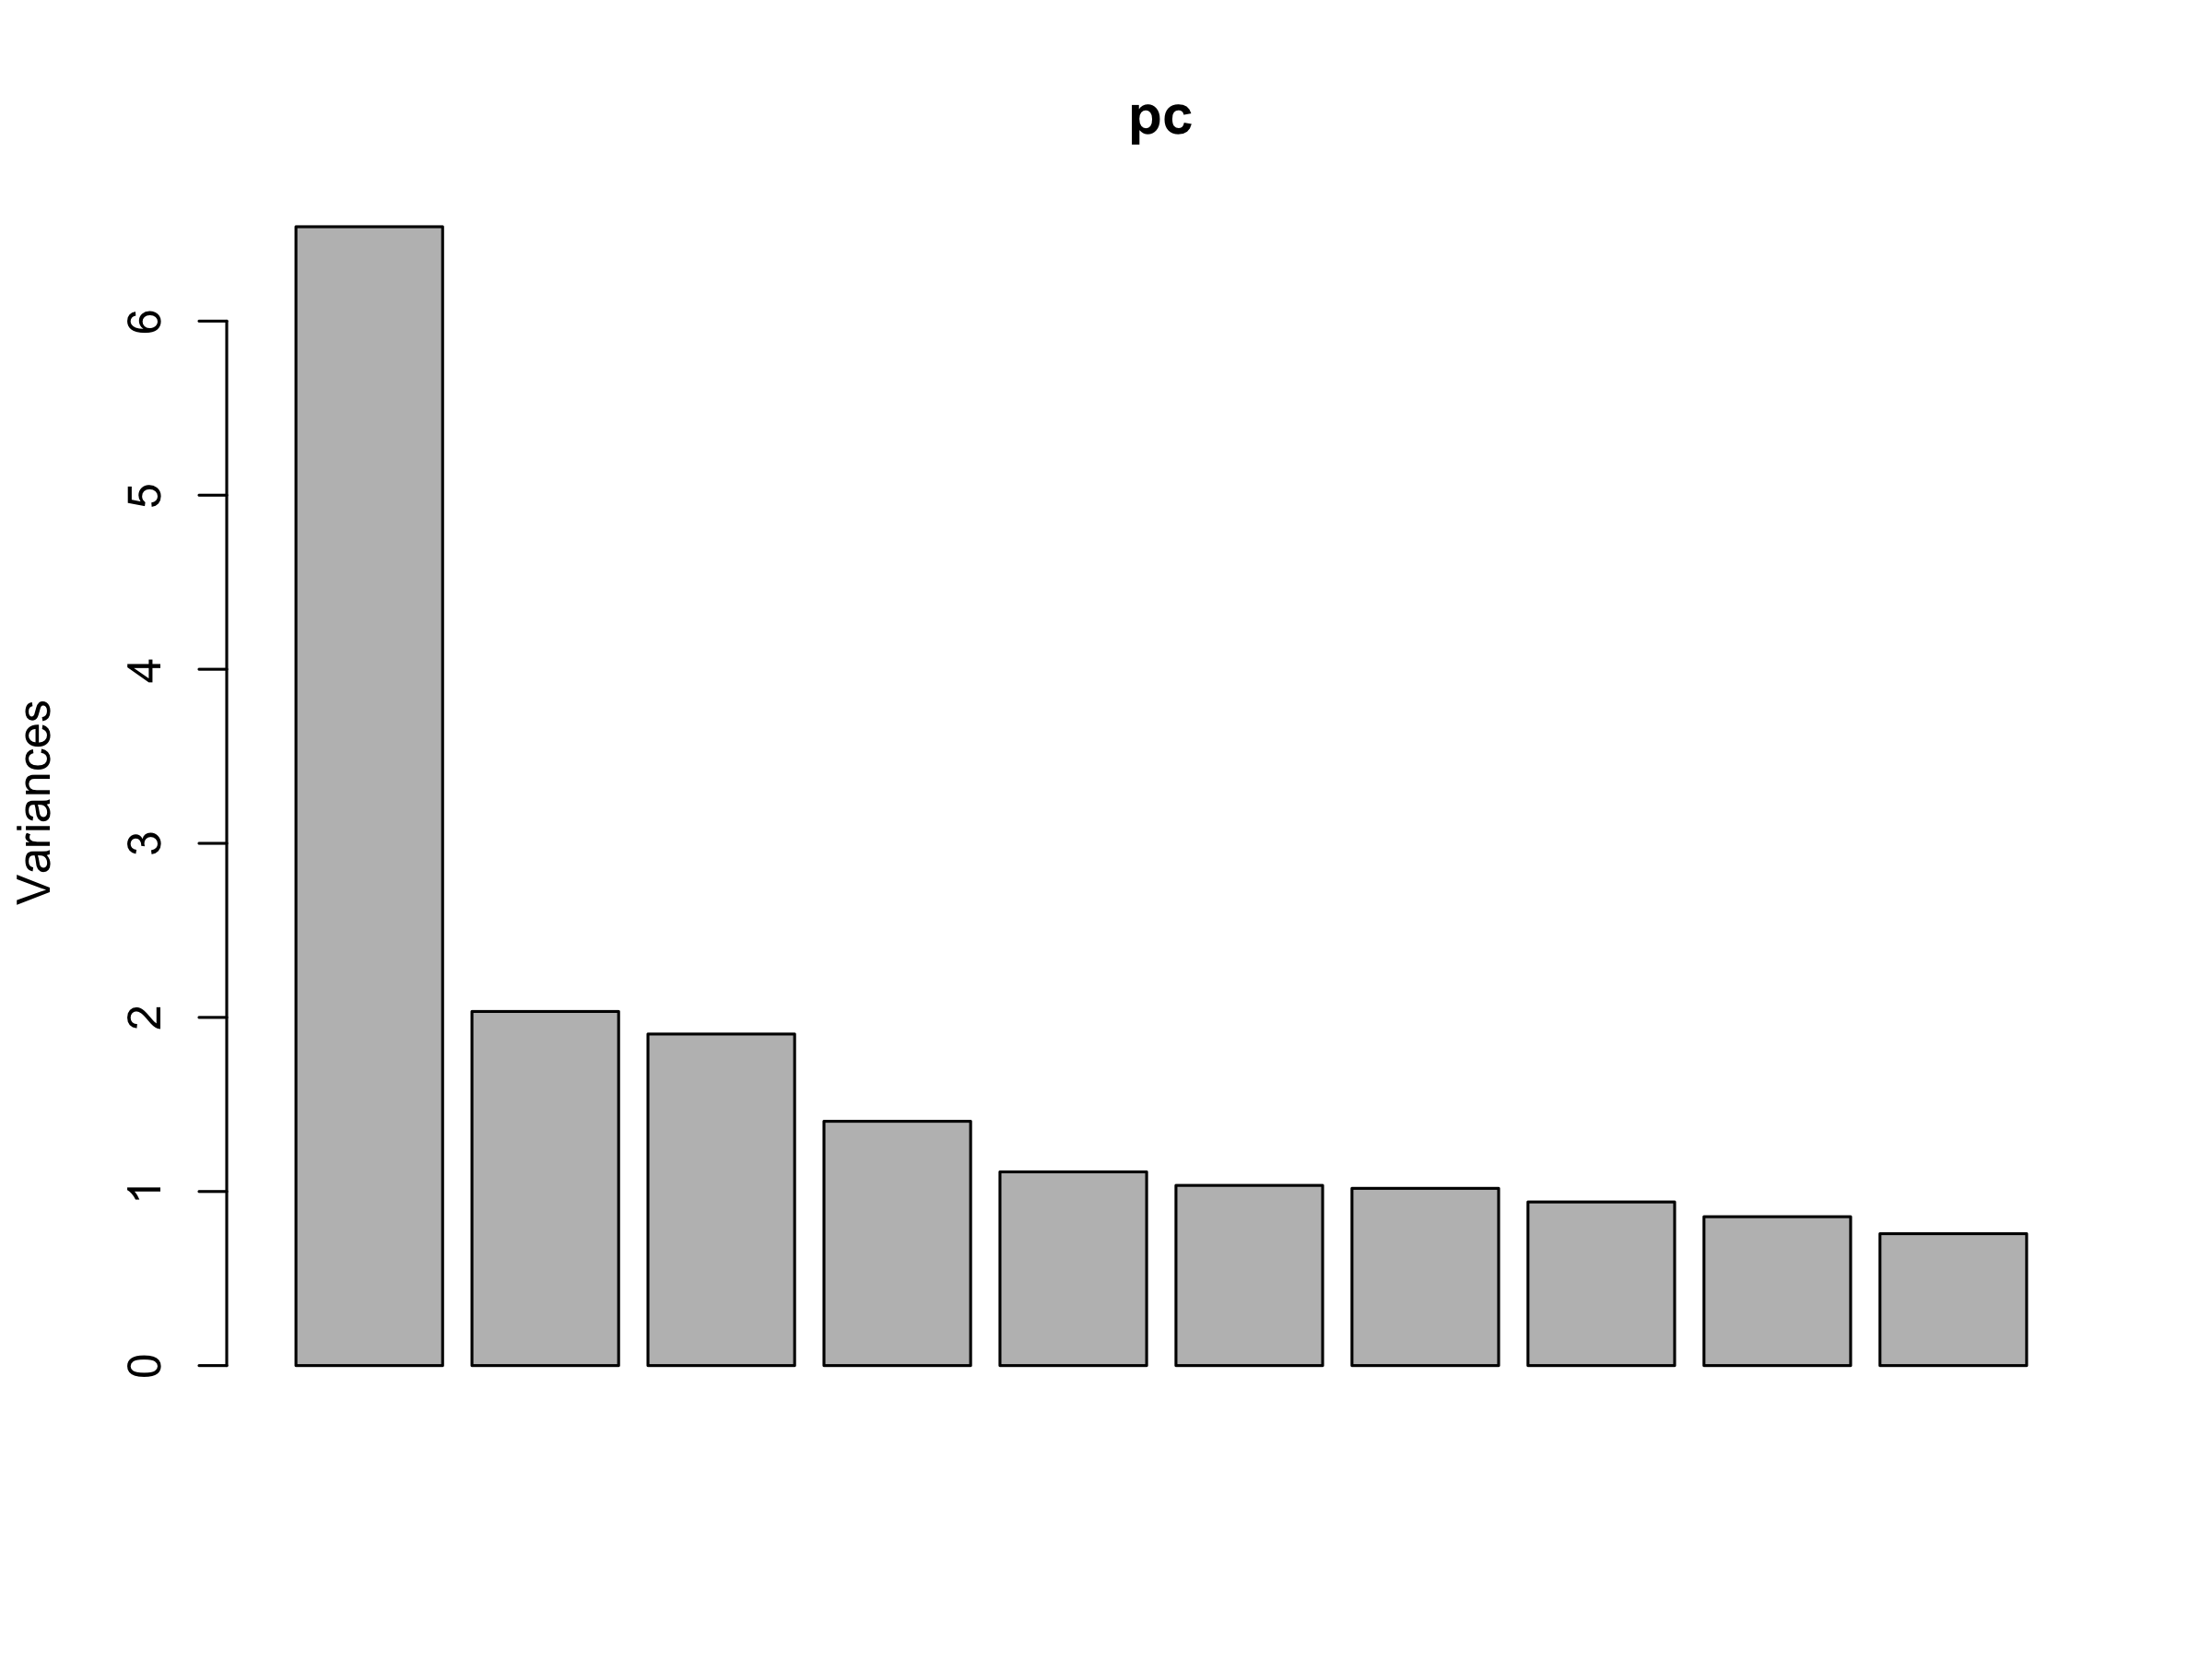
\includegraphics{Report_files/figure-pdf/unnamed-chunk-15-1.png}

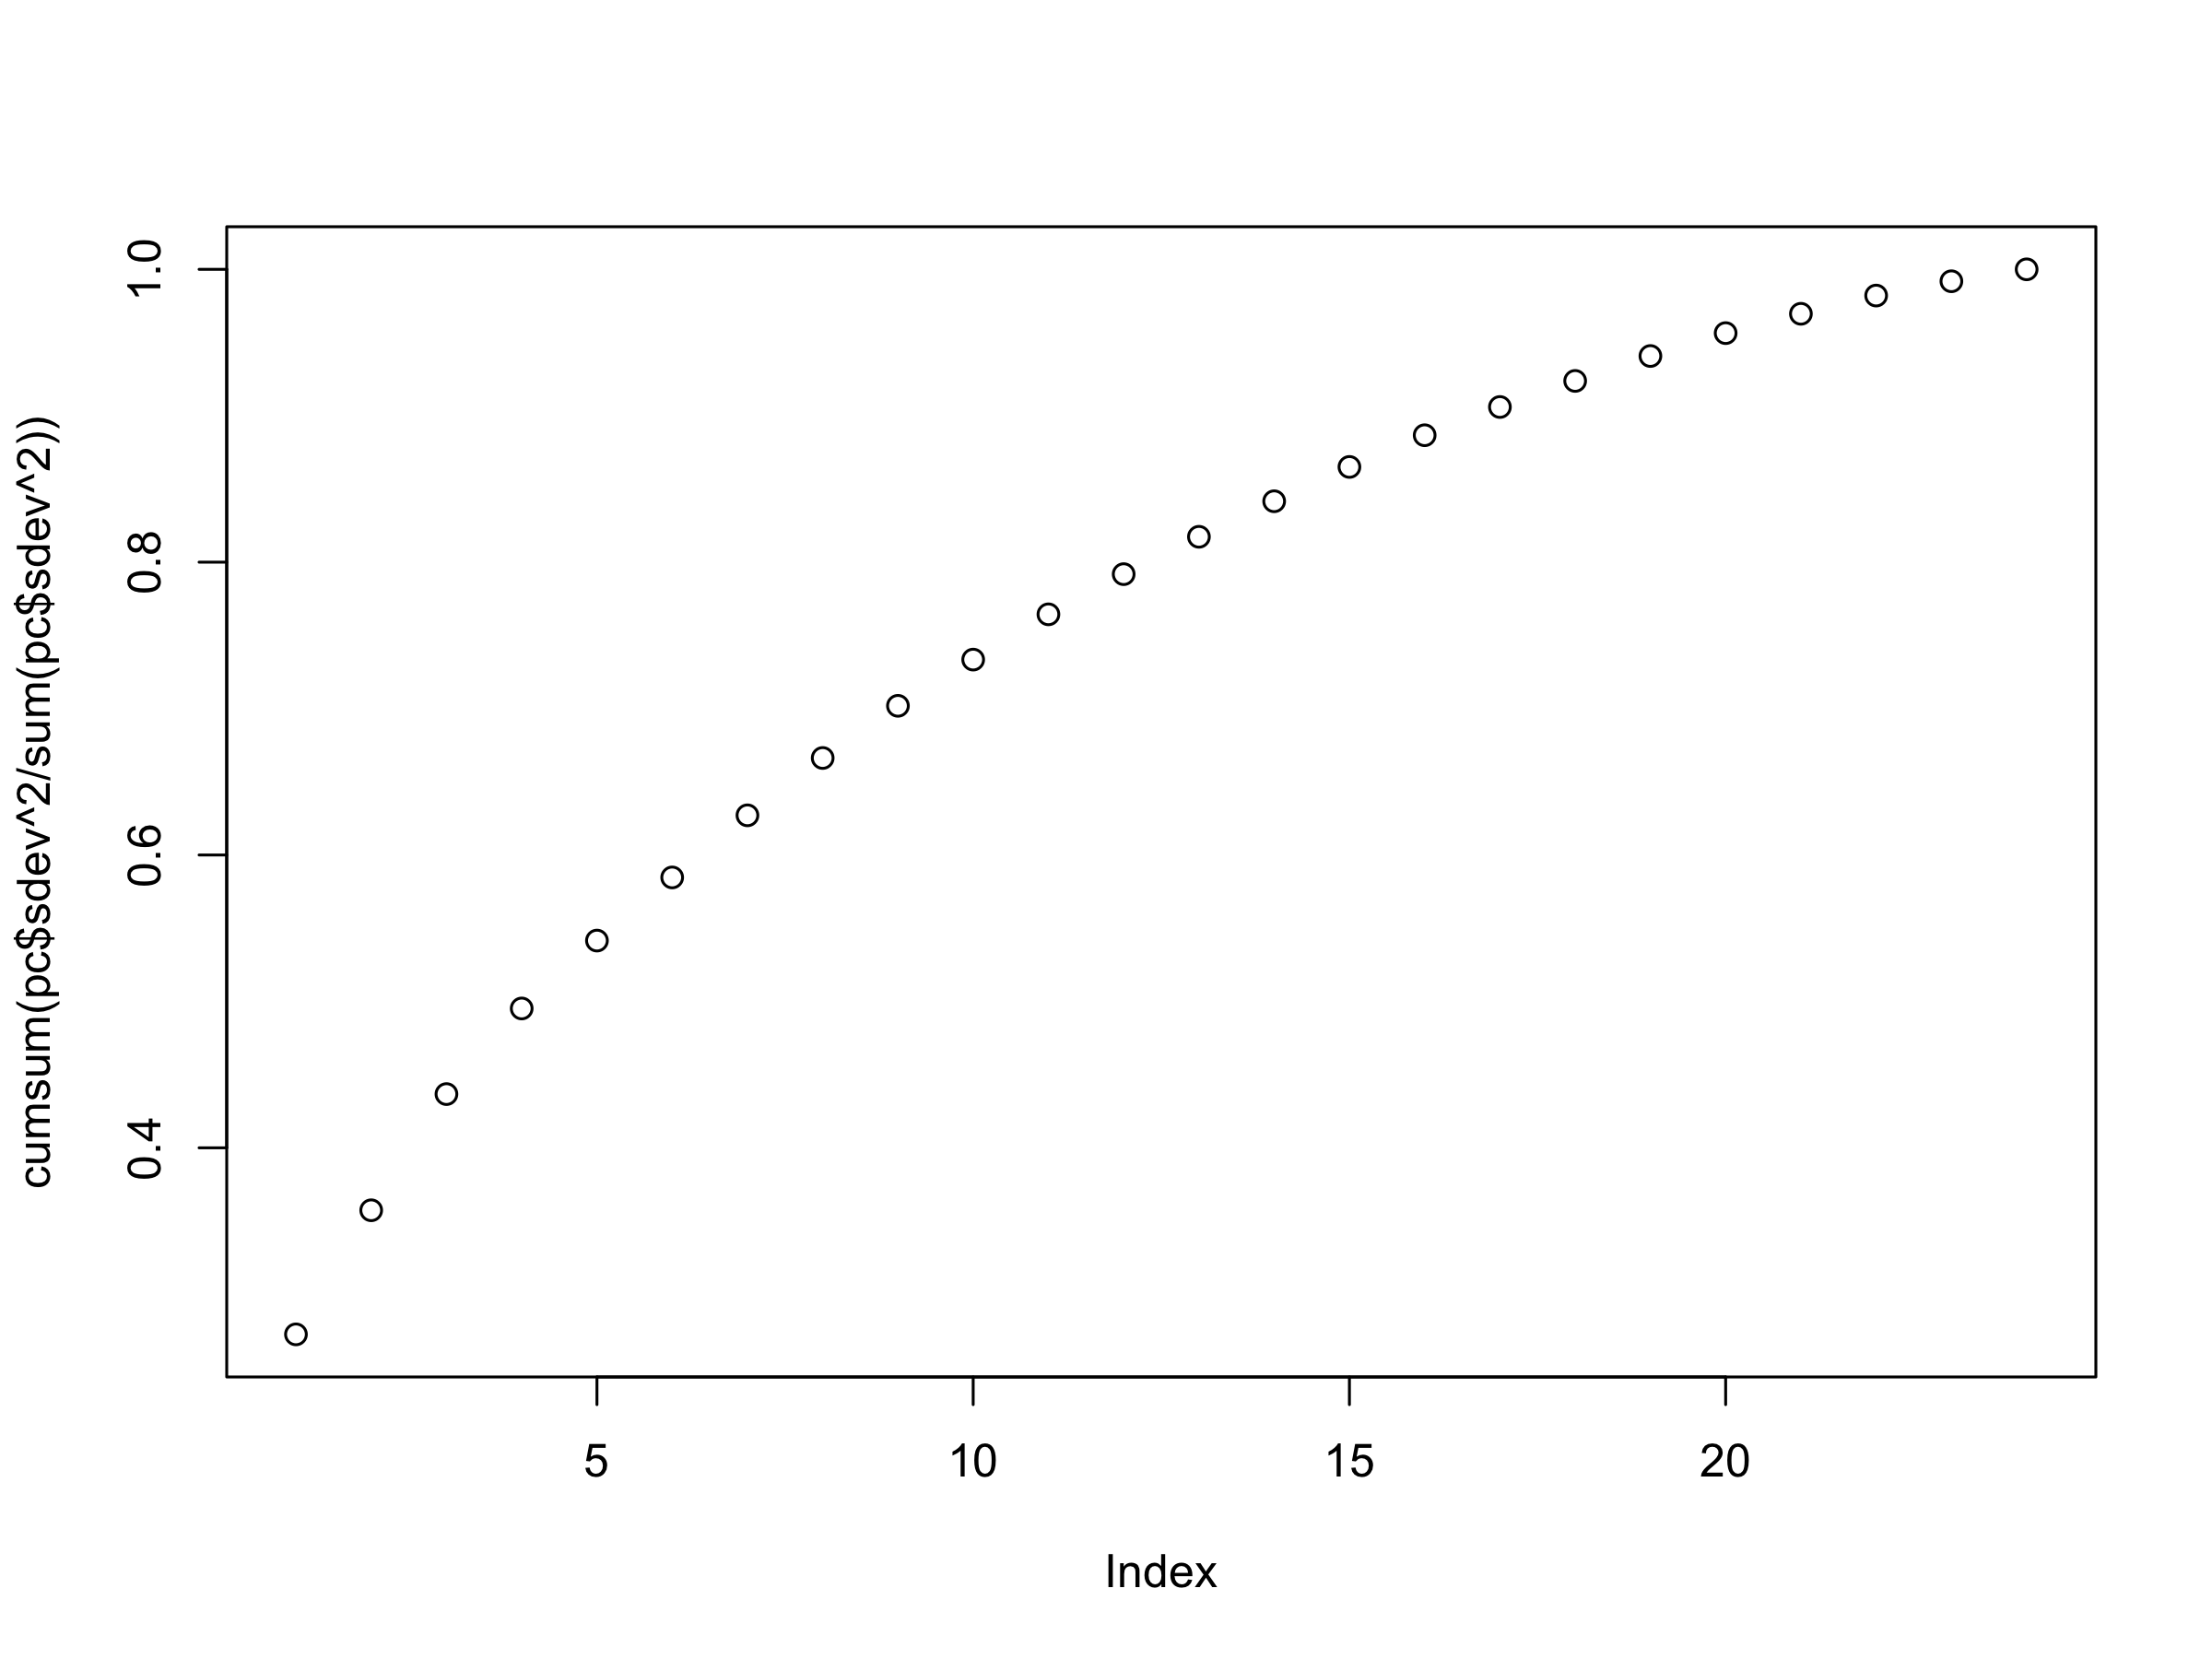
\includegraphics{Report_files/figure-pdf/unnamed-chunk-16-1.png}

Thus, around 13 components are able to explain 80\% variability in the
data.

Below is a plot of the relationship between the first two components
after PCA.

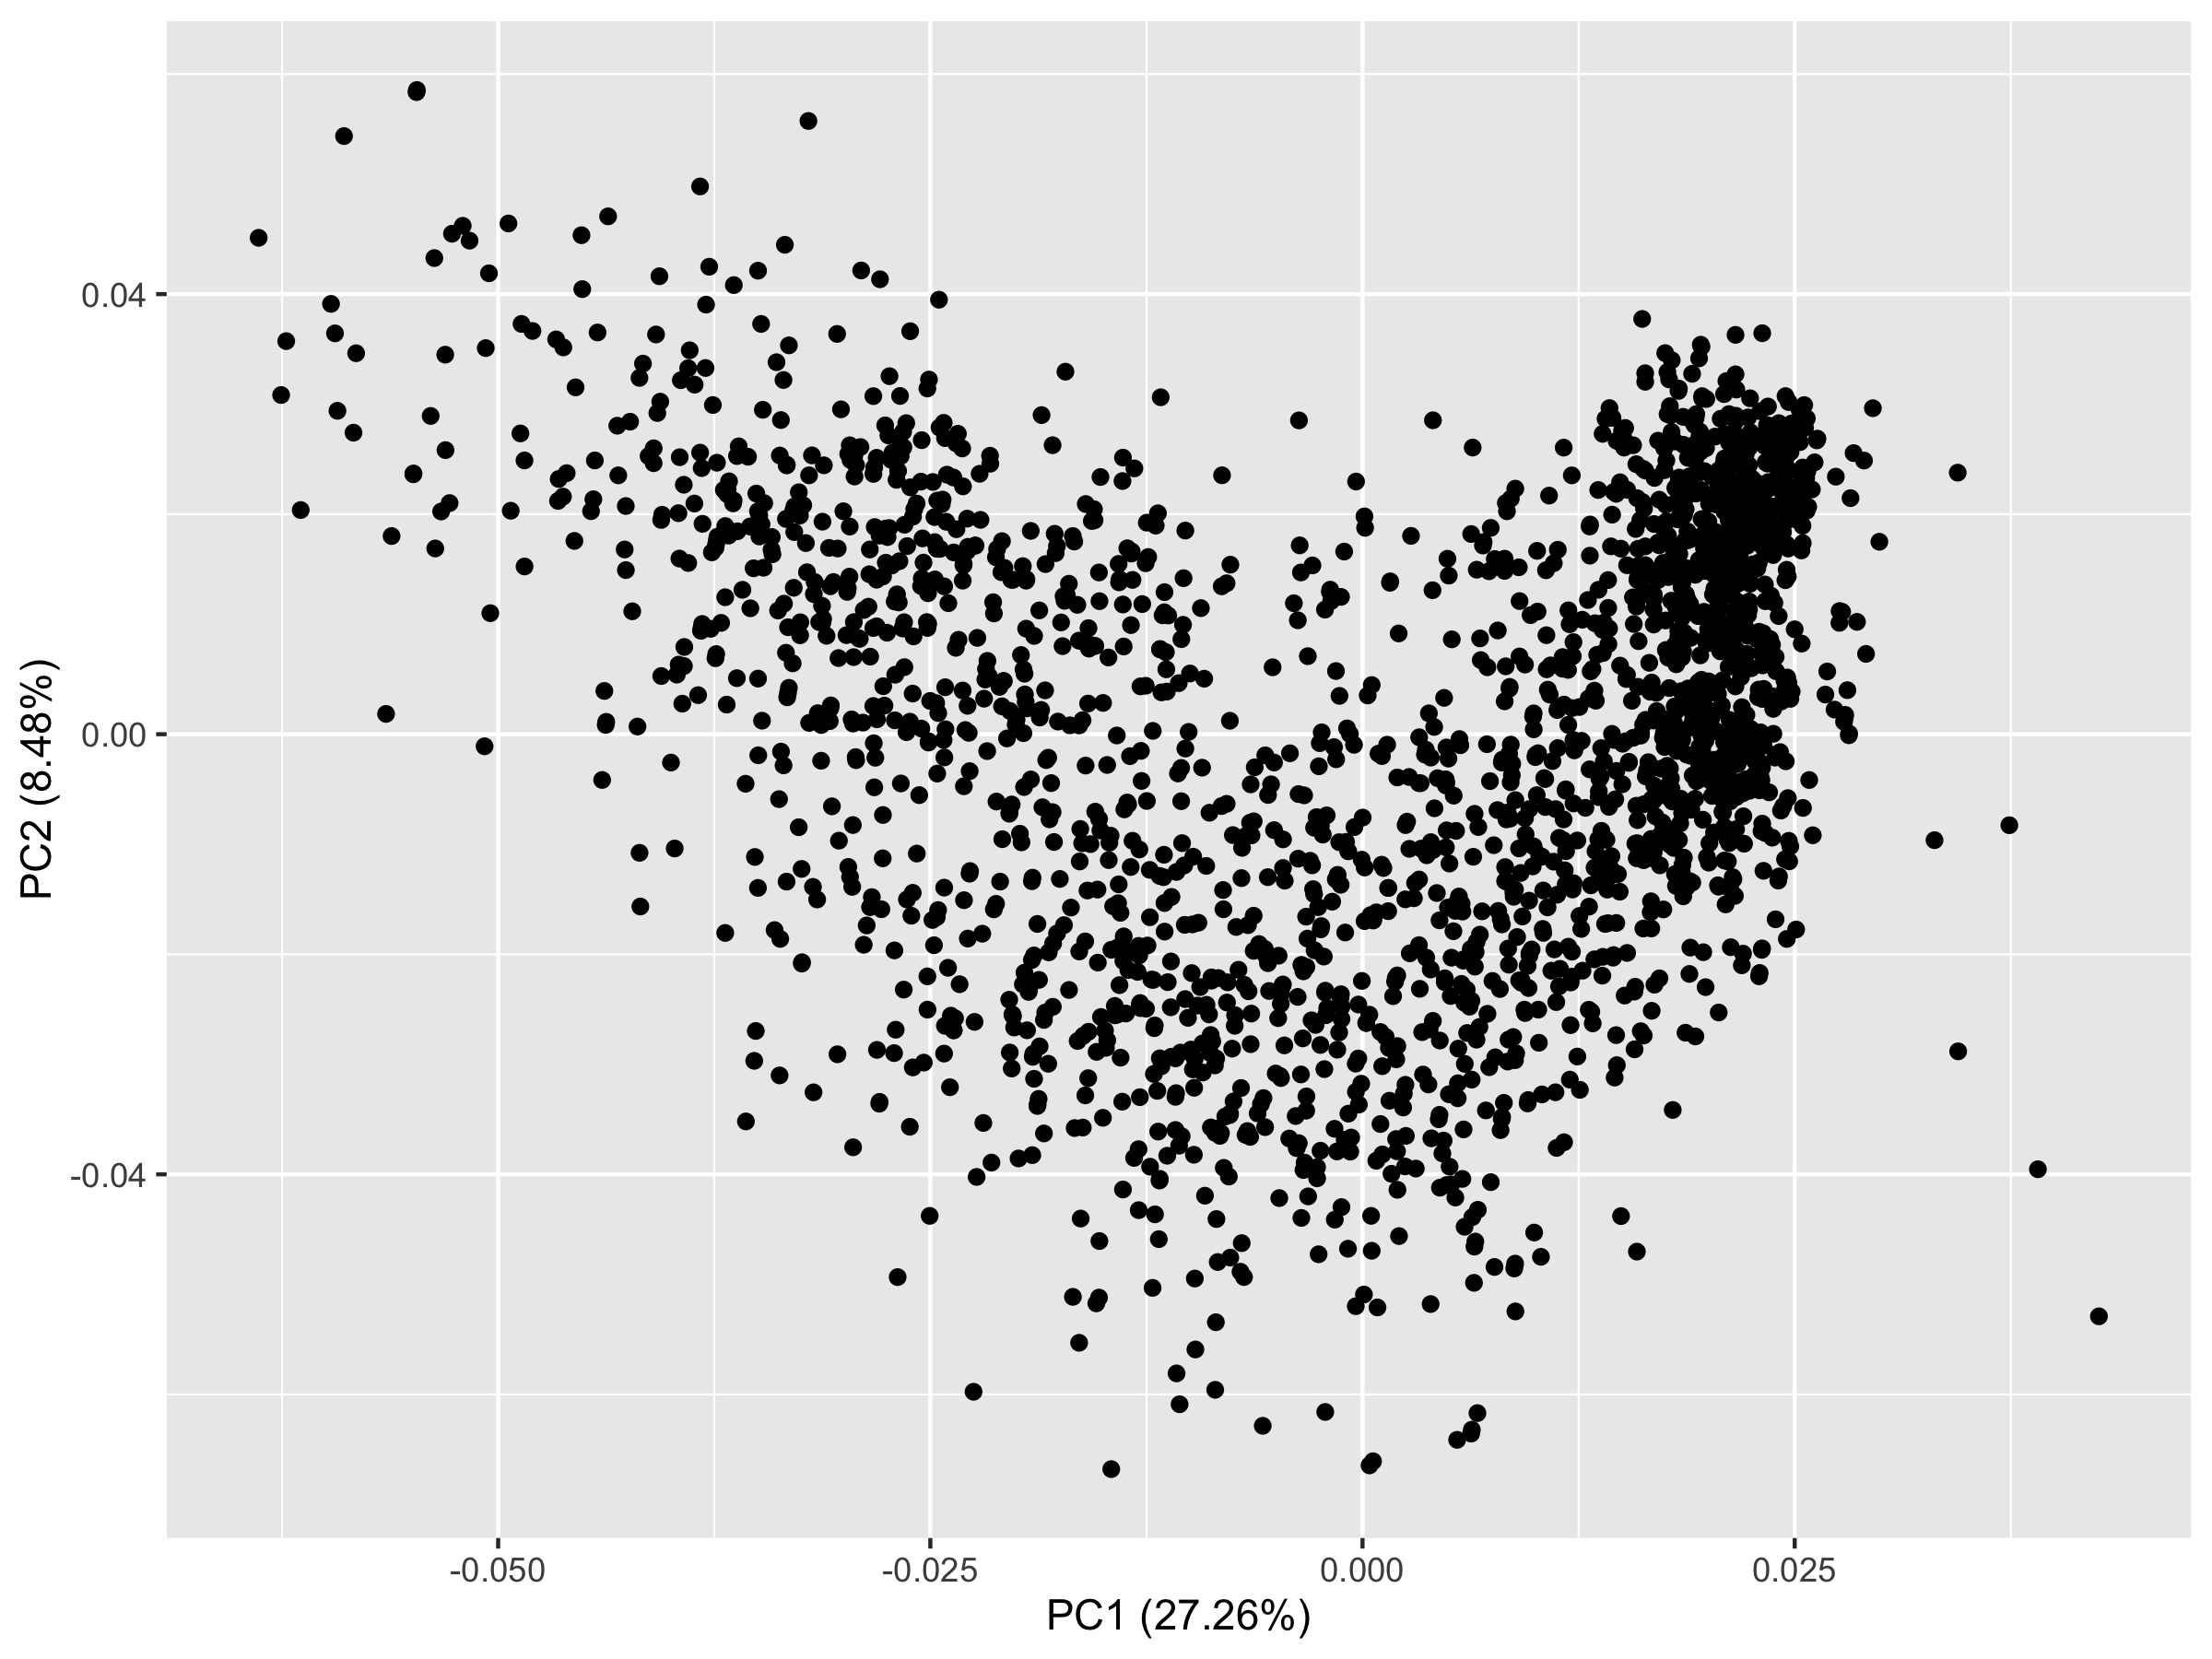
\includegraphics{Report_files/figure-pdf/unnamed-chunk-17-1.png}

Thus, with the help of PCA we can reduce the data with 24 columns to
upto 13 columns and still explain 80\% variability in the data.



\end{document}
